% LGWallRecon -- light-guide inner-wall reconstruction from an entrance-face scan
% Author: Hengne Li (李衡讷) <Hengne.Li@cern.ch>, <Hengne.Li@m.scnu.edu.cn>
%
% User manual, English edition.  Build with build_manual.sh (xelatex).
% Every result number comes from numbers.tex (generated from results/numbers.json).
\documentclass[11pt,a4paper]{article}
\usepackage[a4paper,margin=2.3cm]{geometry}
\usepackage{fontspec}
\usepackage{xeCJK}                         % only for the author's Chinese name
\setCJKmainfont{FandolSong-Regular.otf}
\usepackage{amsmath,amssymb}
\usepackage{graphicx}
\usepackage{booktabs,tabularx,array}
\usepackage{xcolor}
\usepackage{listings}
\usepackage{tikz}
\usetikzlibrary{positioning,arrows.meta}
\usepackage{enumitem}
\usepackage{caption}
\usepackage{float}                         % [H]: keep tables and the pipeline diagram where they are written
\usepackage[hidelinks]{hyperref}

% text shown when a repository URL has not been filled in yet
\newcommand{\UrlPending}{to be added}
% Generated by make_numbers_tex.py from results/numbers.json -- do not edit by hand.
\providecommand{\UrlPending}{to be added}
\newcommand{\Npts}{5029}
\newcommand{\RmsFit}{0.9}
\newcommand{\RmsFitTwo}{0.94}
\newcommand{\RmsIdeal}{5.4}
\newcommand{\ChiTwo}{1.31}
\newcommand{\CorrStruct}{0.98}
\newcommand{\RmsRing}{5}
\newcommand{\LocRms}{13}
\newcommand{\LocMin}{\ensuremath{-}49}
\newcommand{\LocMax}{\ensuremath{+}72}
\newcommand{\MeanMin}{\ensuremath{-}0.95}
\newcommand{\MeanMax}{\ensuremath{-}0.25}
\newcommand{\RAp}{8.47}
\newcommand{\RApDiff}{0.28}
\newcommand{\SpotR}{0.34}
\newcommand{\Amplitude}{0.1320}
\newcommand{\Plateau}{0.0252}
\newcommand{\GfourRatio}{1.0001}
\newcommand{\GfourRatioErr}{0.0013}
\newcommand{\GfourNpoints}{120}
\newcommand{\GfourNphot}{4000}
\newcommand{\GfourPull}{0.98}
\newcommand{\GfourCorr}{0.97}
\newcommand{\RecipRatio}{n/a}
\newcommand{\RecipErr}{n/a}
\newcommand{\ClCorrAll}{0.12}
\newcommand{\ClRmsTrue}{48}
\newcommand{\ClRmsRec}{11}
\newcommand{\ClMapRms}{0.81}
\newcommand{\ClProfErr}{258}
\newcommand{\ResCorrLo}{0.7}
\newcommand{\ResCorrHi}{0.9}
\newcommand{\ResFracVis}{5}
\newcommand{\ResAminLo}{2}
\newcommand{\ResAminHi}{12}
\newcommand{\ResolutionRows}{%
  10 & 1.1 & 0.2 & \ensuremath{+}0.67 \\
  30 & 1.7 & 2.5 & \ensuremath{+}0.92 \\
  60 & 3.2 & 2.9 & \ensuremath{+}0.88 \\
  100 & 6.7 & 4.0 & \ensuremath{+}0.74 \\
  150 & 11.5 & 5.1 & \ensuremath{+}0.71 \\
  200 & 19.2 & 10.1 & \ensuremath{+}0.43 \\
  300 & 41.2 & 14.5 & \ensuremath{+}0.29 \\
  500 & 95.5 & 16.6 & \ensuremath{+}0.25 \\
}
\newcommand{\GithubURL}{\UrlPending}
\newcommand{\GitlabURL}{\UrlPending}


\hypersetup{
  pdftitle={LGWallRecon user manual},
  pdfauthor={Hengne Li (李衡讷), South China Normal University},
  pdfsubject={Light-guide inner-wall reconstruction from an entrance-face scan},
  pdfkeywords={light guide, ray tracing, inverse problem, OpenCL, Geant4}
}
\definecolor{rule}{gray}{0.62}
\definecolor{codebg}{gray}{0.965}
\lstset{basicstyle=\ttfamily\small, columns=fullflexible, keepspaces=true, breaklines=true,
  breakatwhitespace=false, frame=single, framerule=0.3pt, rulecolor=\color{rule},
  backgroundcolor=\color{codebg}, xleftmargin=3pt, xrightmargin=3pt, aboveskip=7pt, belowskip=7pt,
  showstringspaces=false, upquote=true}
\setlist{itemsep=2pt, topsep=4pt}
\setlength{\parskip}{4pt plus 1pt}
\setlength{\parindent}{0pt}
\captionsetup{font=small, labelfont=bf}
\newcolumntype{L}[1]{>{\raggedright\arraybackslash}p{#1}}
\newcolumntype{Y}{>{\raggedright\arraybackslash}X}
\newcommand{\um}{\,\textmu m}
\newcommand{\code}[1]{\texttt{#1}}
\emergencystretch=2em
% one troubleshooting entry: symptom in bold, remedy below
\newcommand{\trouble}[2]{\par\medskip\textbf{#1}\par\nopagebreak #2\par}

\begin{document}

% ------------------------------------------------------------------ title page
\begin{titlepage}
\vspace*{2.5cm}
{\Huge\bfseries LGWallRecon\par}
\vspace{0.5cm}
{\LARGE Light-guide inner-wall reconstruction\\[2pt] from an entrance-face scan\par}
\vspace{0.9cm}
{\Large User manual\par}
\vspace{2.2cm}
{\large Hengne Li (李衡讷)\par}
\vspace{4pt}
South China Normal University\par
\vspace{4pt}
\code{Hengne.Li@cern.ch} \quad \code{Hengne.Li@m.scnu.edu.cn}\par
\vspace{1.2cm}
12 November 2026\par
\vfill
\fbox{\parbox{0.92\textwidth}{\small
\textbf{In one paragraph.} LGWallRecon simulates a hollow conical light guide with a mirror wall by
ray tracing, and searches for a wall shape for which the simulated response map matches a measured
scan of the entrance face. For the scan shipped with the package the simulation and the measurement
differ by \RmsFit\,\% in the inner aperture, against about \NoisePct\,\% point noise. The wall that achieves
this is \emph{not unique}: the scan fixes only a small part of the wall shape. Read the wall figure as
one smooth, regularised solution that explains the scan, not as a survey of the real surface.}}
\end{titlepage}

\tableofcontents
\newpage

% ====================================================================== 1
\section{What the toolkit does}

The light guide is a hollow cone, 17.5\,mm in diameter at the entrance and 8\,mm at the exit,
100\,mm long, lined with reflective film. In the measurement a small diffuse light source is moved
over the entrance face on a $100\times100$ grid with 0.2\,mm step, and a PMT at the exit records the
signal at each position. The result is a two-dimensional response map. It is not flat: it shows an
off-centre dark spot, a bright ring and several bright patches, a few percent in size.

LGWallRecon answers two questions.

\begin{enumerate}
\item \textbf{Can a ray-tracing simulation reproduce this map?} Yes. An ideal cone responds almost
identically at every source position (within $\pm0.2\,\%$, Section~\ref{sec:ideal}), so the
several-percent structure cannot come from an ideal cone; in this model it is attributed to the wall
departing from the ideal shape. With a suitably deformed wall the simulated map agrees with the
measured one to \RmsFit\,\% (rms, inner aperture $r<8$\,mm, \Npts{} scan points); the ideal cone
misses by \RmsIdeal\,\%. The point noise of the measurement is about \NoisePct\,\%.
\item \textbf{Which wall does it?} The toolkit returns one: a deviation field $\delta(\varphi,z)$
from the CAD cone with a local unevenness of \LocRms\um{} rms, largest bump \LocMin\um, largest dent
\LocMax\um, on top of an azimuthal mean deviation between \MeanMax{} and \MeanMin\,mm (the bore is narrower than CAD).
\end{enumerate}

\textbf{The honest headline.} That wall is not the only one. In a closure test a known wall with
seven bumps and dents was turned into a synthetic scan with the measured noise and sent through the
same pipeline. The synthetic map was reproduced down to the noise (residual \ClMapRms\,\%,
$\chi^2/N=\ClChiTwo$), yet the recovered wall is only weakly correlated with the true wall
(\ClCorrAll): true local unevenness \ClRmsTrue\um, recovered \ClRmsRec\um. A linear analysis explains
why. The scan determines some combinations of the wall shape well and most others hardly at all, with
no sharp boundary in between. Inside the 30 best-determined patterns the recovered and the true wall
correlate at \ResCThirty, inside the best 100 at \ResCHundred, inside the best 150 at \ResCOneFifty;
but the test wall has only \ResFThirty\,\%, \ResFHundred\,\% and \ResFOneFifty\,\% of its deformation
power there. The rest is imprinted on the scan too weakly to be recovered.

The measured scan shows the same thing directly. The wall published with an earlier version of this
toolkit, before two corrections of the tracer, still reproduces the scan when it is traced with the
present tracer: to \PrevRmsEarlier\,\%, against \PrevRmsNow\,\% for the present wall. Yet the two
walls are different. Their local unevenness correlates at \PrevCorr{} over the whole wall
(\PrevCorrEntrance{} in the first 20\,mm behind the entrance, nothing further in), and their
azimuthal mean profiles are \PrevProfDiff\um{} RMS apart (Section~\ref{sec:prev}).

\textbf{How to read the wall figure.} It shows \emph{one} regularised solution. The fit penalises
unevenness and starts from an axisymmetric wall, so it tends towards a smooth wall, and it shows that
little unevenness is enough to explain the scan. It is not the only wall that fits, it is not shown
to be the least uneven one that fits, and it does not bound the unevenness of the real wall from
below: reflectivity or detector non-uniformity could produce structure as well. It is not a survey of
the real inner surface. Section~\ref{sec:limits} lists what extra measurements would be needed for
that.

What the package contains:
\begin{itemize}
\item a specular ray tracer for a cone with a free-form wall, on the CPU (\code{numba}) and on the GPU
(OpenCL), tracing the same rays;
\item the inversion pipeline: aperture measurement, axisymmetric profile, linear-response kernels,
damped least-squares inversion with exact residuals;
\item validation tools: self-tests of the ray sequence, of the intersection and of the ideal cone,
Geant4 cross-check, reciprocity test, GPU-against-CPU test, Jacobian test, closure test, resolution
study;
\item figure, table and report generators in Chinese and English, including a single-file web page
with a live 3-D demonstration of rays in the guide.
\end{itemize}

Figure~\ref{fig:wall} shows the wall returned for the shipped scan and Figure~\ref{fig:maps} the
comparison of the simulated with the measured map.

\begin{figure}[p]
\centering
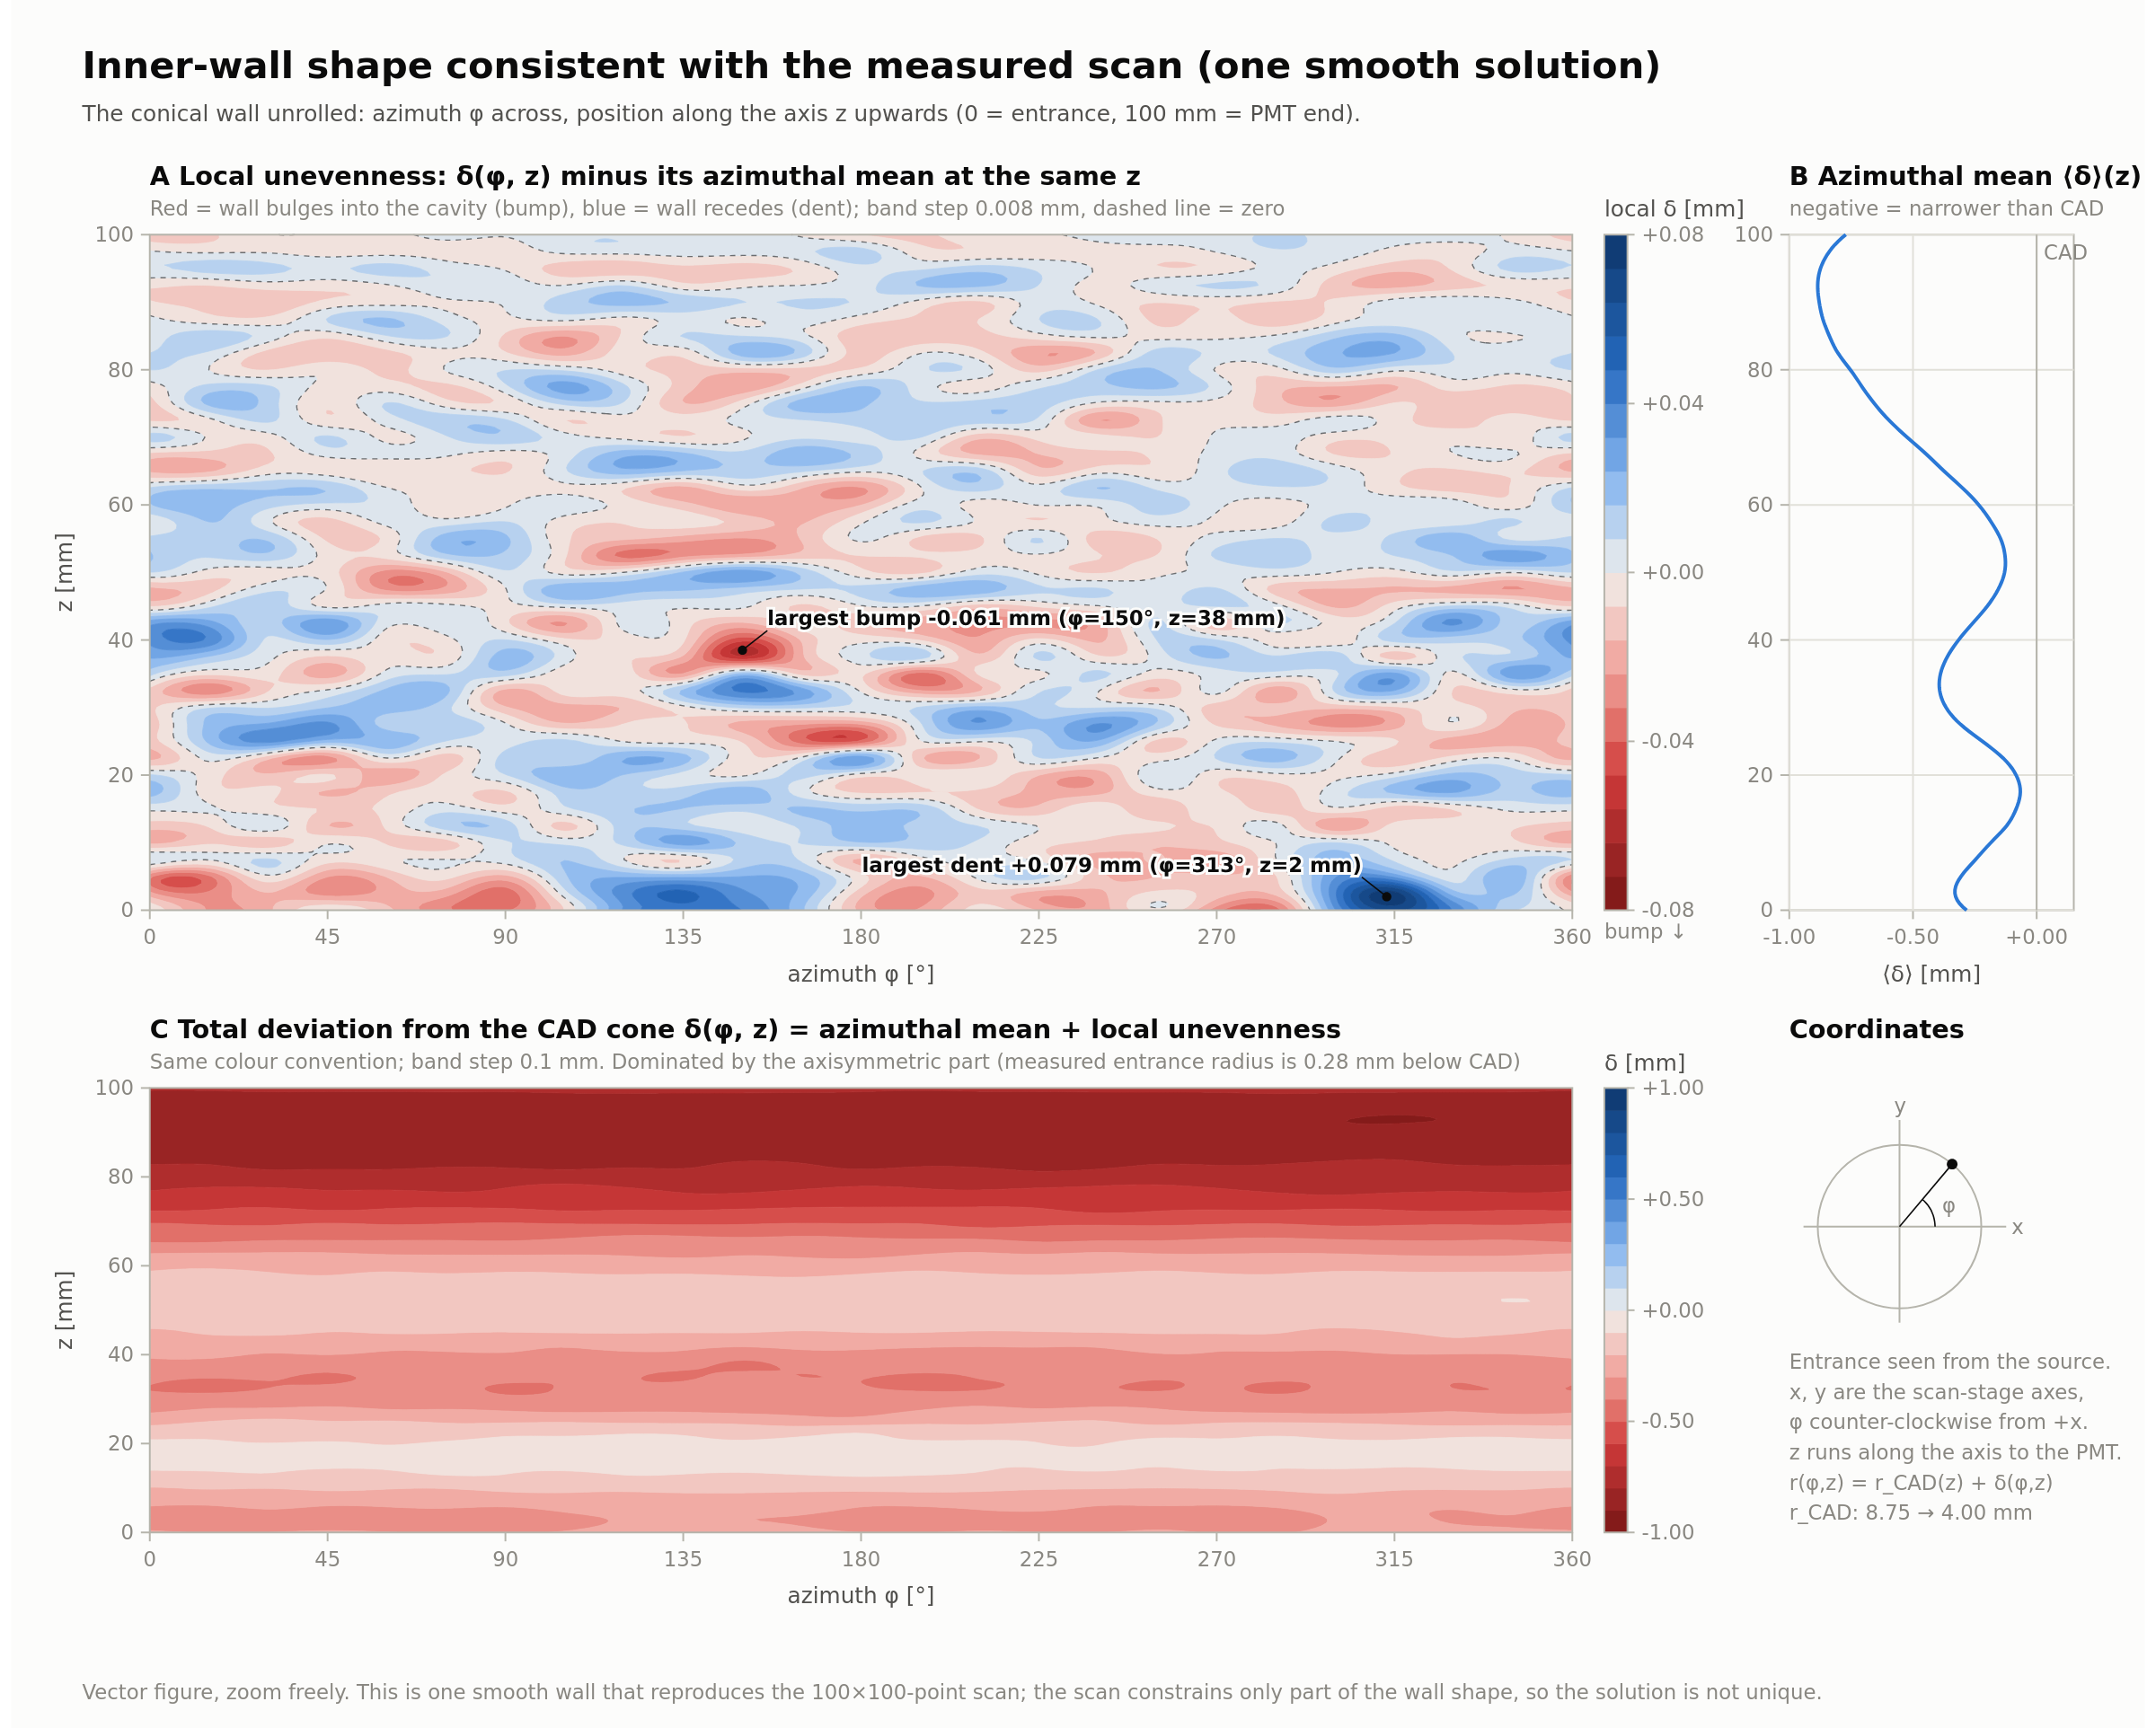
\includegraphics[width=0.88\textwidth]{fig/en/inner_surface.png}
\caption{The wall figure (\texttt{inner\_surface.svg}). A: local unevenness, the deviation minus its
azimuthal mean. B: the azimuthal mean. C: the total deviation from the CAD cone. Red is a bump into
the cavity, blue a dent.}\label{fig:wall}
\end{figure}

\begin{figure}[p]
\centering
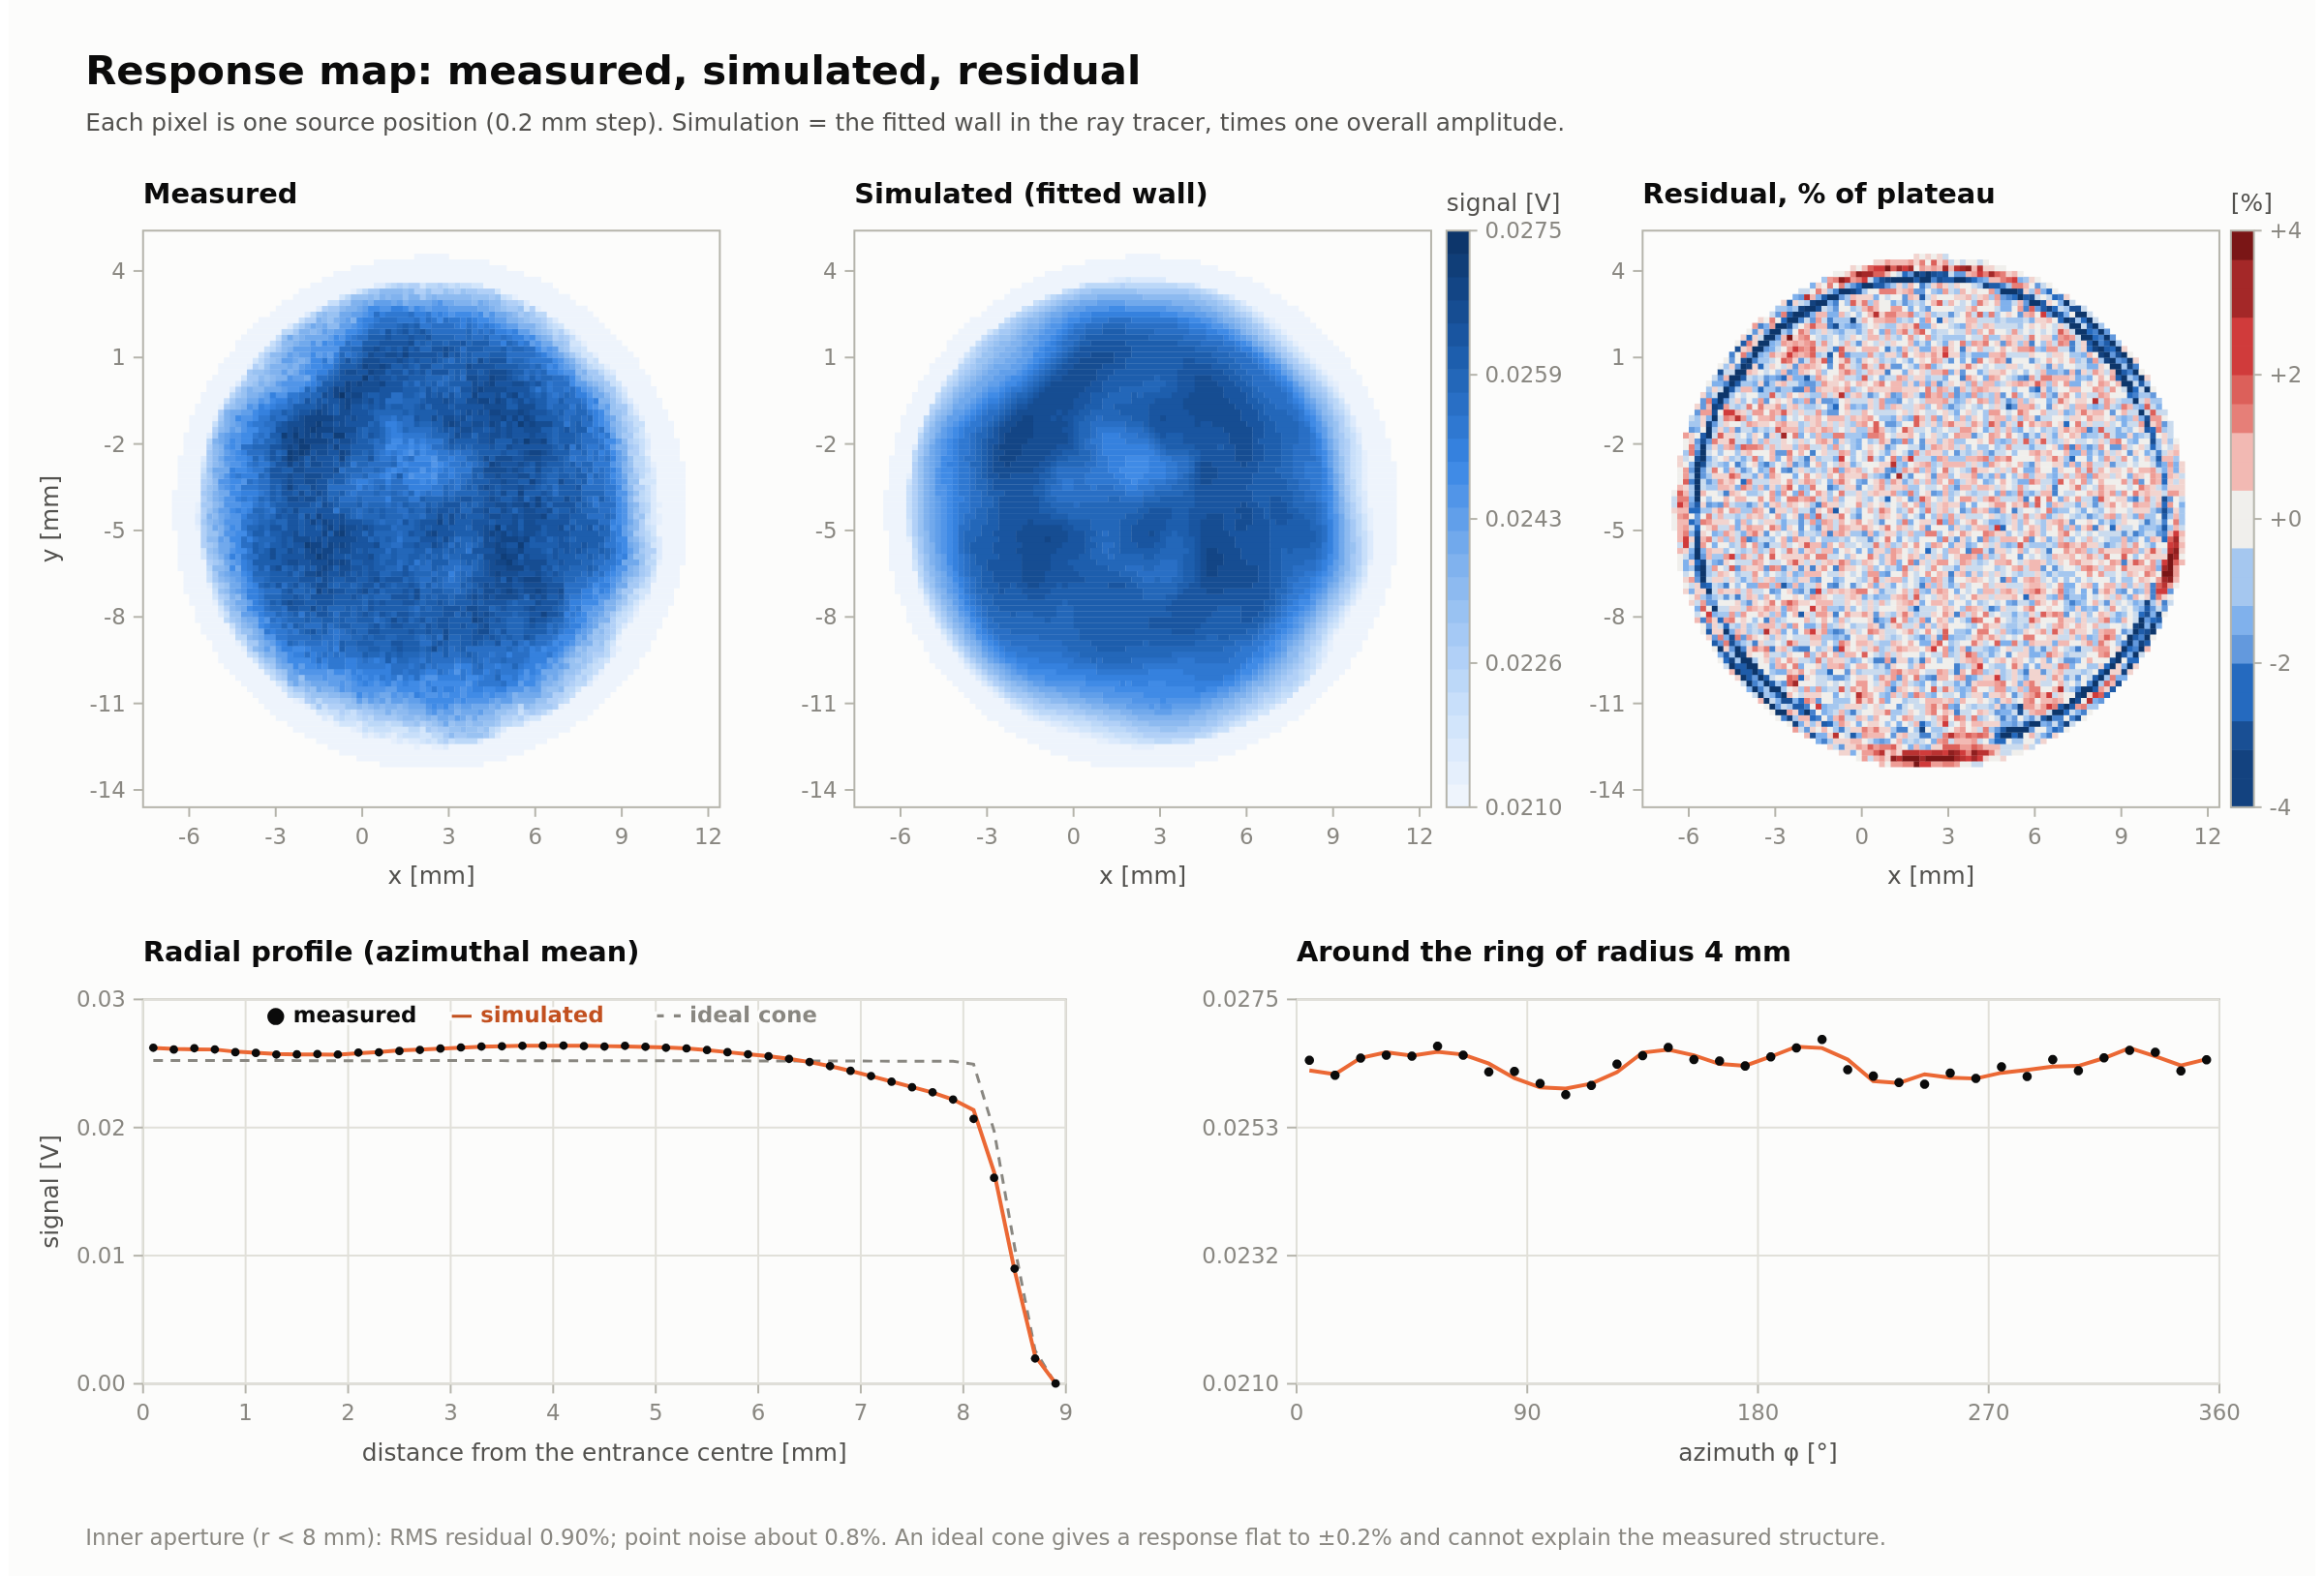
\includegraphics[width=0.88\textwidth]{fig/en/response_maps.png}
\caption{Measured map, simulated map and residual (\texttt{response\_maps.svg}), with the azimuthally
averaged radial profile and the signal around the ring of radius 4\,mm.}\label{fig:maps}
\end{figure}

\clearpage

% ====================================================================== 2
\section{Physics and model}

\subsection{Geometry and coordinates}

All lengths are in millimetres. The $z$ axis is the optical axis, $z=0$ at the entrance plane and
$z=L=100$ at the exit plane where the PMT sits. The nominal (CAD) wall radius is
\[
  r_\mathrm{CAD}(z) = R_1 + (R_2-R_1)\,\frac{z}{L}, \qquad R_1 = 8.75,\quad R_2 = 4.00,
\]
a cone of half angle $2.72^\circ$. The real wall is written as
\[
  r(\varphi,z) = r_\mathrm{CAD}(z) + \delta(\varphi,z).
\]
$\delta<0$ means the wall bulges into the cavity (a bump); $\delta>0$ means it recedes (a dent).

The transverse axes $x,y$ are the scan-stage axes, with the origin moved to the measured centre of the
entrance aperture. The azimuth $\varphi$ is counted counter-clockwise from $+x$, looking at the
entrance from the light-source side. Relating $\varphi$ to the hardware requires knowing how the stage
axes are oriented with respect to the light guide, and which of the four cells of the block was
scanned; the toolkit cannot know either.

The CAD file \path{data/4cells_17.5mm_8mm_circle_to_circle_100mm-Cut.step} describes a block with four
identical cells. Each cell is the cone above followed by a cylindrical pocket of 16.36\,mm diameter
and 10\,mm depth that holds the PMT. Only the cone enters the simulation.

\subsection{Source, wall and detector}

\begin{description}[leftmargin=1.6em]
\item[Source] A small spot in the entrance plane that emits like a Lambertian surface into the
forward hemisphere. The spot is a uniform disc; its radius (\SpotR\,mm for the shipped scan) is
measured from the sharp edge of the scan. Rays that start outside the aperture are blocked.
\item[Wall] A perfect mirror: specular reflection with reflectivity 1. A reflectivity below 1 can be
set (parameter \code{refl}) and was tried as a free parameter of the axisymmetric fit. Starting from
the perfect-mirror fit, freeing the reflectivity moves it to \ReflFit, and $\chi^2$ falls from
\ReflChiFixed{} to \ReflChi{} (\ReflNpts{} points, one more parameter); the wall profile changes its
shape but keeps its size. Reflectivity and profile are strongly degenerate and this scan cannot
separate them, so results are quoted for a perfect mirror.
\item[Detector] Every ray that crosses the exit plane $z=L$ inside the wall is counted, whatever its
angle and position. A ray that returns through the entrance plane is lost.
\end{description}

The simulated signal at source position $(x,y)$ is $A\,T(x,y)$, where $T$ is the fraction of all
emitted light that reaches the exit and $A$ is one overall amplitude (volts per unit transmission)
fitted to the data. The absolute scale of the measurement is therefore not used.

\subsection{The ideal cone}
\label{sec:ideal}

For a Lambertian source the ideal cone has a simple response. Averaged over the entrance area, the
transmission equals the area ratio exactly,
\[
  \langle T_\mathrm{ideal}\rangle = \left(\frac{R_2}{R_1}\right)^2 = 0.2090 .
\]
This is conservation of \'etendue: a lossless concentrator cannot pass more than the area ratio of a
Lambertian input, and the cone reaches that limit because every ray started backwards from the exit
reaches the entrance.

At a single source position the transmission is only nearly that value. A reflection off the cone
conserves the closest approach of a ray to the apex, so whether a ray gets through is decided by a
sphere centred on the apex that passes through the exit rim. The exit, however, is a flat disc and
not that spherical cap. The transmission therefore falls slowly from $+0.22\,\%$ at the centre to
about $-0.14\,\%$ at the rim, relative to the area ratio. An earlier version of this manual called
the response exactly flat; it is flat to $\pm0.2\,\%$.

The tracer reproduces the area average within the tolerance of its self-test ($2\times10^{-4}$,
relative) and Geant4 agrees with the tracer along a radius (Section~\ref{sec:validation}). The
consequence for the inversion: the several-percent structure of the measured map cannot come from an
ideal cone. In this model it is attributed to the wall being non-ideal; effects outside the model
could contribute as well (Section~\ref{sec:limits}).

\subsection{The wall as a B-spline surface}

$\delta(\varphi,z)$ is a tensor-product uniform cubic B-spline,
\[
  \delta(\varphi,z) = \sum_{i=0}^{N_\varphi-1}\;\sum_{j=0}^{N_z+2} c_{ij}\,B_i^{(\varphi)}(\varphi)\,B_j^{(z)}(z).
\]
In $\varphi$ the spline is periodic with $N_\varphi=24$ knots at $\varphi_i = 2\pi i/N_\varphi$
($15^\circ$ apart). In $z$ there are $N_z$ cells on $[0,L]$ and $N_z+3$ coefficients; coefficient $j$
is centred at $z_j=(j-1)\,L/N_z$, so the first and the last one sit one cell outside the guide. The
final fit uses $N_z=40$ (2.5\,mm cells, 43 coefficients per azimuth), which gives $24\times43=1032$
wall parameters. The spline is $C^2$, so the surface normal is continuous, which specular reflection
needs.

\subsection{Ray--wall intersection}
\label{sec:intersection}

A ray $\mathbf p+t\,\mathbf d$ hits the wall where
$f(t)=\sqrt{x^2+y^2}-r_\mathrm{CAD}(z)-\delta(\varphi,z)$ changes sign from negative to positive. The
tracer finds the first such $t$ in three steps.
\begin{enumerate}
\item \emph{Bounding cones and the wall zone.} $\delta$ lies between two numbers $\delta_\mathrm{lo}$
and $\delta_\mathrm{hi}$ (sampled on a fine grid, with a small margin). The wall therefore lies
between the cones $r_\mathrm{CAD}+\delta_\mathrm{lo}$ and $r_\mathrm{CAD}+\delta_\mathrm{hi}$, whose
intersections with the ray are roots of a quadratic. Only the part of the ray inside this thin
\emph{wall zone} can hit the wall. The part inside the inner cone is skipped analytically, which
leaves at most two intervals of $t$ to search.
\item \emph{Marching with the derivative.} Each interval is walked in steps of at most 0.5\,mm, and
both $f$ and its derivative $f'$ along the ray are sampled. A change of sign of $f$ brackets a hit.
If $f'$ changes from positive to negative between two samples, $f$ has a maximum in between; the
maximum is located by regula falsi on $f'$ and tested. A grazing hit that enters and leaves the wall
within one step is therefore not skipped.
\item \emph{Illinois regula falsi} on the bracket, to $10^{-10}$\,mm in double precision
($2\times10^{-6}$\,mm in single precision).
\end{enumerate}
A hit can now be missed only if $f$ has two extrema inside one 0.5\,mm step, which needs structure far
below the size of a spline cell (2.5\,mm along $z$, at least 1\,mm along the arc).

Earlier versions marched the whole bracket in 3\,mm steps and looked for a sign change of $f$ only;
such a march can step over a grazing hit. \code{test\_grazing\_hit.py} holds a case that it missed:
a ray 11\um{} inside the nominal cone and a ring-shaped bump of 11.3\um, which the ray penetrates by
0.3\um{} over 0.7\,mm of path. On the wall published with that version the 3\,mm march, the present
march and a 0.02\,mm march gave identical transmissions for $2\times10^{7}$ rays, so the published
numbers were not affected.
The outward normal is the gradient of $F=r-r_\mathrm{CAD}(z)-\delta(\varphi,z)$,
\[
  \mathbf n \;\propto\; \hat{\mathbf r} \;-\; \frac{1}{r}\frac{\partial\delta}{\partial\varphi}\,\hat{\boldsymbol\varphi}
  \;-\;\Big(\frac{R_2-R_1}{L}+\frac{\partial\delta}{\partial z}\Big)\hat{\mathbf z},
\]
with the derivatives taken analytically from the spline, and the ray is reflected as
$\mathbf d' = \mathbf d-2(\mathbf d\cdot\mathbf n)\,\mathbf n$. A ray ends when it crosses $z=L$
(detected) or $z=0$ (lost).

\subsection{Quasi-random rays and common random numbers}

For a Lambertian source the direction cosines $(d_x,d_y)$ are uniform in the unit disc. Only
directions with $\sin\theta\le s_\mathrm{max}$ are sampled, because steeper rays never reach the exit
(for the fitted wall nothing is lost with $s_\mathrm{max}=0.5$; the pipeline uses 0.55), and the
result is scaled by $s_\mathrm{max}^2$.

Rays are quasi-random rather than random. The four numbers that define a ray (two for the direction,
two for the position inside the spot) come from the $R_4$ additive recurrence
$u_j(k)=\operatorname{frac}(s_j+k\,g^{-j})$, $j=1\ldots4$, with $g=1.1673039782614187$, the real root
of $x^5=x+1$. The numbers $1,g^{-1},\ldots,g^{-4}$ are linearly independent over the rationals, so
the points fill the unit 4-cube evenly. The recurrence is evaluated in 32-bit integer arithmetic so
that the CPU and the GPU produce the same rays. The two extra coordinates of the optional blur of the
spot use $\sqrt2-1$ and $\sqrt3-1$. Each source position has its own shifts $s_j$ (a
Cranley--Patterson rotation derived from a hash of the point index and a seed).

\emph{Corrected in this version.} Earlier versions used the root of $x^4=x+1$, for which
$g^{-3}+g^{-4}=1$ exactly. The two spot coordinates were then locked together and the spot was
sampled along a spiral instead of over the disc, with its centroid displaced by 0.12 spot radii in a
direction that changed from point to point. This acted as extra model noise (0.22\,\% of $T$ instead
of 0.10\,\% at 20\,000 rays per point), not as a bias (mean shift $4\times10^{-5}$).
\code{test\_sampler.py} now checks that no integer relation with small coefficients holds between
the constants, that every pair of coordinates fills a $32\times32$ grid evenly, and that the centroid
of the sampled spot sits at its centre.

The chain was rerun from the start with both corrections (the march of
Section~\ref{sec:intersection} and this one). The fit quality changed little ($\chi^2/N$ from 1.31 to
\ChiTwo), but the wall that came out is a different one (Section~\ref{sec:prev}).

Two properties follow from the quasi-random rays.
\begin{itemize}
\item The noise of $T$ falls faster than $1/\sqrt{N}$: with 20\,000 rays per point it is about
0.1\,\% of $T$, where independent random rays would give about 1.5\,\%.
\item For a fixed seed the map is a deterministic function of the wall. Differences between two
walls are then computed with \emph{common random numbers}: most rays have the same fate in both, and
the noise of the difference is far below the noise of either map. All finite differences and all
fit iterations rely on this.
\end{itemize}

\subsection{How a patch of wall shows up in the scan}

A small deformation at height $z$ and azimuth $\varphi$ does not change the response near the point
on the entrance face ``below'' it. It changes the fate of the marginal rays, those that just make it
to the exit or just fail to, and for a given wall patch these rays come from a thin arc of source
positions. The arc is typically 0.5\,mm wide, and its position and radius change quickly with $z$:
patches near the entrance affect sources at the adjacent rim, patches around mid-length draw arcs
and rings a few millimetres from the centre, patches near the exit give diffuse rings. The picture
resembles tomography, with each scan pixel summing wall deformations along a curve.

Two practical consequences: the response is very sensitive (a deformation of order 0.03\,mm changes
the map by a few percent), and it needs a fine axial resolution of the wall model (2.5\,mm cells)
to place the arcs correctly.

\subsection{The inversion}
\label{sec:inversion}

The fit minimises the objective
\[
  Q(c,A) = \sum_n \frac{\big(d_n-A\,T_n(c)\big)^2}{\sigma^2}
  + \lambda^2\,\lVert P c\rVert^2 + (0.05\,\lambda)^2\,\lVert c-c_\mathrm{base}\rVert^2
  + \sum_i \frac{\big(\delta(\varphi_i,0)-\delta_\mathrm{ap}(\varphi_i)\big)^2}{(0.005\ \mathrm{mm})^2}.
\]
$d_n$ are the pedestal-subtracted scan values inside the fit radius (8\,mm by default), $\sigma$
combines the point noise ($2.0\times10^{-4}$\,V) with the Monte Carlo noise of the model, $P$ takes
first differences of the coefficients along $\varphi$ and $z$ (a smoothness penalty), $c_\mathrm{base}$
is the axisymmetric base wall, and the last term ties the wall radius at $z=0$ to the aperture
radius measured from the edge of the scan (in a closure test, to the aperture of the synthetic wall).
The first term is the data $\chi^2$; the printed $\chi^2/N$ refers to it alone. The second and third
terms penalise unevenness and distance from the base wall, in the metric of the spline coefficients;
$Q$ is not the surface RMS of the wall under a fit tolerance.

$T_n(c)$ is not differentiable in closed form, and a brute-force finite-difference Jacobian is too
noisy for single spline coefficients. The package uses two devices.

\emph{Fourier-mode kernels.} Around an axisymmetric base wall the response to an azimuthal mode
$\delta c_{ij}=a\cos(m\varphi_i)$ at one $z$ knot is a sum of a few harmonics
$\sum_q A_{jmq}(\rho)\cos(q\psi)$ of the source azimuth $\psi$, with $q\in\{m,\,N_\varphi-m,\,N_\varphi+m\}$.
One run perturbs the whole circumference, so the signal is strong while the wall slopes stay small, and
projecting on $\cos(q\psi)$ averages the noise over all source angles. Central differences remove the
second-order term. The Jacobian for any single coefficient follows by Fourier synthesis and rotation.
Against exact finite changes of the map (Section~\ref{sec:jactest}) these kernels reach a correlation
of \JacCorrMin--\JacCorrMax{} and a slope of \JacSlopeMin--\JacSlopeMax{} for non-axisymmetric
perturbations of 10--100\um{} RMS. For changes of the azimuthal mean profile they are poor: the
correlation is \JacBumpCorrMin--\JacBumpCorrMax{} for a gentle bump and
\JacStepCorrMin--\JacStepCorrMax{} for a sharp step. A smooth deformation is the small remainder of
large single-knot responses that cancel, so errors of a few percent in the single-knot kernels become
errors of order one for smooth shapes.

\emph{Damped iterations with exact residuals.} Each Levenberg--Marquardt step solves the linearised
problem with a damping term $\mu\lVert\Delta c\rVert^2$, then evaluates the true $Q$ with a full
ray trace. The step is kept if $Q$ falls (and $\mu$ is halved); otherwise $\mu$ is multiplied by
four and the step is recomputed, up to eight times. A Broyden rank-one update corrects the Jacobian
with what each trial step actually did to the map. Because the residual is always exact, every
accepted step really lowers $Q$, whatever the errors of the kernels.

That does not mean the best fit is reached. The iteration stops when eight successively more damped
trial steps all fail to lower $Q$, which is a practical stopping rule and not a proof of a minimum.
The result is one regularised solution; it depends on the start wall, on the regularisation weights
and on the approximate Jacobian. Two earlier fits of the shipped scan, with earlier versions of the
code, ended at $\chi^2/N=1.48$ and 1.31; the present one ends at \ChiTwo.

The axisymmetric part of the wall is large (tenths of a millimetre) and non-linear, so the chain
first fits an axisymmetric profile alone (Stage A), then runs two rounds of kernels and inversion,
the second with kernels recomputed around the updated azimuthal mean.

% ====================================================================== 3
\section{Installation}

\subsection{Requirements}

\begin{tabularx}{\textwidth}{@{}L{3.6cm}Y@{}}
\toprule
Component & Needed for \\
\midrule
Python $\ge 3.10$ with \code{numpy}, \code{scipy}, \code{matplotlib}, \code{numba},
\code{contourpy}, \code{pillow} & everything \\
\code{pyopencl} and an OpenCL GPU & fast tracing (optional, \path{requirements-gpu.txt}; without it use \code{LG\_GPU=0}) \\
Geant4 11.x, CMake, a C++17 compiler & the independent cross-check in \code{g4/} (optional) \\
Node.js & the animated ray figure \code{ray\_animation.svg} (optional) \\
TeX Live with \code{xelatex} and \code{ctex} & rebuilding this manual (optional) \\
Firefox & rendering the manual figures from SVG (optional) \\
Linux with \code{systemd} user sessions & the resource wrapper \code{tools/run\_limited.sh} \\
\bottomrule
\end{tabularx}

\subsection{Python environment}

\begin{lstlisting}
git clone <repository url> LGWallRecon
cd LGWallRecon
python3 -m venv .venv
.venv/bin/python -m pip install --upgrade pip
.venv/bin/python -m pip install -r requirements-gpu.txt   # with the GPU tracer (adds pyopencl)
.venv/bin/python -m pip install -r requirements.txt       # or: CPU only
\end{lstlisting}
\path{requirements.txt} lists what a CPU-only installation needs; \path{requirements-gpu.txt}
includes it and adds \code{pyopencl}, which needs a working OpenCL driver.

The scripts expect the interpreter at \path{.venv/bin/python} relative to the package root. The
shell drivers accept another interpreter through the variable \code{PY}.

\subsection{GPU (optional but recommended)}

The tracer runs on any OpenCL device that \code{pyopencl} can see. Check with
\begin{lstlisting}
clinfo -l
.venv/bin/python -c "import pyopencl as cl; print([d.name for p in cl.get_platforms() for d in p.get_devices()])"
\end{lstlisting}
The development machine has an AMD Radeon 8060S (Ryzen AI Max+ 395) driven through ROCm 7.2; the
device appears as \code{gfx1151} on the platform ``AMD Accelerated Parallel Processing''. On AMD
hardware \code{nvidia-smi} is absent and says nothing about GPU availability; use \code{clinfo} or
\code{rocminfo}.

Measured speeds for the fitted wall:

\begin{tabularx}{\textwidth}{@{}L{6.2cm}Y@{}}
\toprule
Configuration & Rays per second \\
\midrule
GPU, single precision (default) & about $2.4\times10^{7}$ (measured while the machine was busy) \\
GPU, double precision & roughly 10--30 times slower than single \\
CPU, double precision (\code{numba}) & of order $10^{5}$ per core \\
\bottomrule
\end{tabularx}

The GPU version traces tens of millions of rays per second, roughly an order of magnitude faster than
the CPU version on all cores of this machine. The wall-zone march with the derivative
(Section~\ref{sec:intersection}) costs about a factor 1.6 on the GPU against the plain 3\,mm march of
earlier versions, which reached $3.8\times10^{7}$ rays per second. The kernel is single precision; its
result for every source point was checked against the CPU in double precision
(Section~\ref{sec:validation}). Without a GPU everything still runs with \code{LG\_GPU=0}; expect the
full chain to take many hours instead of about 50 minutes.

Integrated GPUs share the system memory, and a cgroup memory limit does not cap GPU allocations. The
tracer keeps its buffers at a few megabytes and submits work in slices of about half a second, so it
neither exhausts memory nor trips the driver watchdog.

\subsection{Geant4 (optional)}

\begin{lstlisting}
source <geant4 prefix>/bin/geant4.sh
cd g4 && mkdir -p build && cd build
cmake .. -DCMAKE_PREFIX_PATH=<geant4 prefix>
make -j4
\end{lstlisting}
This builds \path{g4/build/lgsim}. No Geant4 data sets beyond the standard installation are needed;
the program uses a minimal physics list with optical photons, transportation and the optical boundary
process only.

% ====================================================================== 4
\section{Quick start}

\begin{lstlisting}
cd LGWallRecon
./run_all.sh
\end{lstlisting}

\code{run\_all.sh} first runs three self-tests of the tracer (\code{test\_sampler.py},
\code{test\_grazing\_hit.py}, \code{test\_ideal\_cone.py}), then measures the aperture, runs the
reconstruction chain on \path{data/scan_summary.csv}, compares the GPU with the CPU on the fitted
wall (if the GPU is on), compares the fitted wall with the wall of an earlier fit of the same scan
(\code{compare\_walls.py}, Section~\ref{sec:prev}), exports the wall, draws the figures in both
languages and assembles the report pages. Every heavy step goes through \path{tools/run_limited.sh}
(Section~\ref{sec:resources}). The drivers run with \code{set -euo pipefail}: a failing step or
self-test stops the run.
\begin{lstlisting}
./run_all.sh --with-checks
\end{lstlisting}
also runs the closure test with the resolution study, the reciprocity test, the Jacobian test, the axisymmetric fit with
a free mirror reflectivity and, if Geant4 is installed, the Geant4 cross-check.

Measured run times with the GPU, on a machine that was busy with other jobs: 48 minutes for the
chain from the aperture to the final map, most of it in the two kernel computations (about 22 minutes
each). The checks take about two hours more: the closure test about 60 minutes, the reciprocity test
about 22 minutes, Geant4 (both runs, with the mesh) about 40 minutes. An idle machine is faster.

Where the results appear:

\begin{tabularx}{\textwidth}{@{}L{5.6cm}Y@{}}
\toprule
Path & Content \\
\midrule
\path{results/en/inner_surface.svg}, \path{results/zh/...} & the wall figure (vector, zoomable) \\
\path{results/<lang>/response_maps.svg} & measured map, simulated map, residual, profiles \\
\path{results/<lang>/closure.svg} & closure test (after \code{closure.sh}) \\
\path{results/<lang>/ray_animation.svg} & animated side view of traced rays \\
\path{results/wall_delta.csv} & $\delta(\varphi,z)$ on a $1^\circ\times0.5$\,mm grid \\
\path{results/wall_coeffs.json} & the B-spline coefficients \\
\path{results/numbers.json} & every number quoted in the report and in this manual \\
\path{docs/LGWallRecon_report_en.html}, \path{..._zh.html} & single-file report pages with the 3-D demonstration \\
\path{out/} & intermediate \code{.npz} and \code{.log} files (not versioned) \\
\bottomrule
\end{tabularx}

To run the stages by hand, change into \path{src/} first; the scripts use paths relative to it.
\begin{lstlisting}
cd src
R=../tools/run_limited.sh; PY=../.venv/bin/python
$R $PY edge.py && $R $PY edge_spot.py      # aperture and light spot -> ../out/edge.npz
$R ./pipeline.sh data                      # the reconstruction chain, log in ../out/pipeline_data.log
$R ./make_report.sh ../out/final_data.npz  # exports, figures, report pages
\end{lstlisting}

% ====================================================================== 5
\section{The pipeline, step by step}
\label{sec:pipeline}

\begin{figure}[H]
\centering
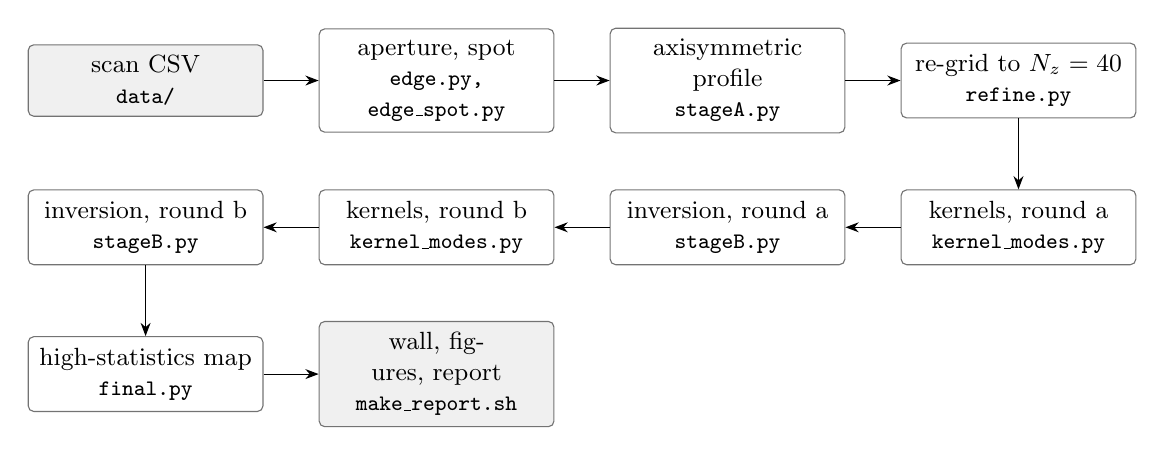
\begin{tikzpicture}[node distance=5mm and 7mm, >=Stealth,
  box/.style={draw=black!55, rounded corners=2pt, align=center, font=\small, inner sep=4pt, minimum height=9mm, text width=27mm},
  io/.style={box, fill=black!6}]
\node[io] (scan) {scan CSV\\ \footnotesize\ttfamily data/};
\node[box, right=of scan] (edge) {aperture, spot\\ \footnotesize\ttfamily edge.py, edge\_spot.py};
\node[box, right=of edge] (A) {axisymmetric profile\\ \footnotesize\ttfamily stageA.py};
\node[box, right=of A] (ref) {re-grid to $N_z=40$\\ \footnotesize\ttfamily refine.py};
\node[box, below=9mm of ref] (k1) {kernels, round a\\ \footnotesize\ttfamily kernel\_modes.py};
\node[box, left=of k1] (b1) {inversion, round a\\ \footnotesize\ttfamily stageB.py};
\node[box, left=of b1] (k2) {kernels, round b\\ \footnotesize\ttfamily kernel\_modes.py};
\node[box, left=of k2] (b2) {inversion, round b\\ \footnotesize\ttfamily stageB.py};
\node[box, below=9mm of b2] (fin) {high-statistics map\\ \footnotesize\ttfamily final.py};
\node[io, right=of fin] (out) {wall, figures, report\\ \footnotesize\ttfamily make\_report.sh};
\draw[->] (scan) -- (edge); \draw[->] (edge) -- (A); \draw[->] (A) -- (ref); \draw[->] (ref) -- (k1);
\draw[->] (k1) -- (b1); \draw[->] (b1) -- (k2); \draw[->] (k2) -- (b2); \draw[->] (b2) -- (fin); \draw[->] (fin) -- (out);
\end{tikzpicture}
\caption{The reconstruction chain. \texttt{pipeline.sh} runs the boxes from \texttt{stageA.py} to
\texttt{final.py}.}
\end{figure}

All commands below are run from inside \path{src/}, through \path{../tools/run_limited.sh}.
Environment variables used by the scripts are collected in Table~\ref{tab:env}.

\subsection{\texttt{edge.py}: the entrance aperture}

\begin{lstlisting}
python edge.py
\end{lstlisting}
The edge of the scan is sharp, so the aperture can be measured directly, without ray tracing. The
script takes the pedestal as the median signal far outside the aperture ($r>10$\,mm), then fits the
radial edge profile in 48 azimuthal sectors with a plateau level, a slope and an error-function edge.
The centre is moved until the $m=1$ Fourier component of the edge radius vanishes. Output:
\path{../out/edge.npz} with the centre, the pedestal and the Fourier coefficients ($m=0\ldots8$) of
the edge radius $r_\mathrm{ap}(\varphi)$, and a diagnostic plot \path{../out/edge.png}.

For the shipped scan the mean radius is \RAp\,mm, that is \RApDiff\,mm below the CAD value of
8.75\,mm, with $m=2$ and $m=4$ components of about 0.03\,mm.

The first guess of the centre and the radial window of the edge fit are constants near the top of
the script; change them for a different aperture (Section~\ref{sec:adapt}).

\subsection{\texttt{edge\_spot.py}: the light spot}

\begin{lstlisting}
python edge_spot.py
\end{lstlisting}
A global fit of all edge points compares a Gaussian spot with a uniform disc. The disc describes the
edge better (the signal has no tail outside the aperture). The script adds the disc radius
(\SpotR\,mm) and a small correction of the mean aperture radius to \path{../out/edge.npz}. All later
stages read the spot from that file.

\subsection{\texttt{stageA.py}: the axisymmetric profile}

\begin{lstlisting}
LG_TAG=data python stageA.py 10 fix 3.0
LG_TAG=refl LG_START=../out/A_data.npz python stageA.py 10 refl 3.0
\end{lstlisting}
Arguments: number of $z$ cells $N_z$ (10), \code{fix} or \code{refl} (fit the mirror reflectivity as
well), weight of the curvature penalty (3.0). With \code{LG\_START=<A\_*.npz>} the fit starts from the
profile of an earlier Stage-A fit and from a reflectivity of 1, so a fit with the reflectivity free
can only improve on the perfect-mirror fit it starts from and the two $\chi^2$ can be compared
(second line; this is what \code{run\_all.sh --with-checks} runs). The reflectivity is capped at 1 and
its derivative is taken as a backward difference. The script fits an axisymmetric wall offset
$\delta_0(z)$ and the amplitude to the azimuthally averaged radial profile of the scan
($\rho=0.1\ldots7.9$\,mm), by Levenberg--Marquardt with finite differences and common random numbers
(120\,000 rays per radius). The radius at $z=0$ is tied to the measured aperture. Output:
\path{../out/A_<tag>.npz} and a plot.

How to judge it: the printed ``data'' $\chi^2$ should fall by more than an order of magnitude from the
start value, and the residual plot should stay within about $\pm1\,\%$ of the plateau. The profile
itself is \emph{not} well determined: different runs return visibly different $\delta_0(z)$ with
the same fit quality (Section~\ref{sec:limits}).

\subsection{\texttt{refine.py}: re-gridding along $z$}

\begin{lstlisting}
python refine.py ../out/A_data.npz 40 ../out/start_data.npz
\end{lstlisting}
Re-expresses a wall on a different number of $z$ cells. The input is either a Stage-A result (the
profile is copied to all 24 azimuthal knots) or a fitted wall. For nested grids ($10\to40$) the
conversion is exact.

\subsection{\texttt{kernel\_modes.py}: the linear response}

\begin{lstlisting}
python kernel_modes.py ../out/start_data.npz 24 dataa 12000 0.06
\end{lstlisting}
Arguments: a wall file (its azimuthal mean becomes the base wall), $N_\varphi$, a tag, rays per source
point (12\,000), mode amplitude $a$ in mm (0.06; mode $m$ uses $\min(a,\,0.18/m)$, which caps the
wall slope of the high modes; in \code{pipeline.sh} the amplitude is set with \code{LG\_KAMP}). Sources sit on a
polar grid of 57 radii (0.075 to 8.475\,mm) and 49 angles on the half circle. For each of the 43 $z$
knots and each mode $m=0\ldots12$ the script traces the wall with $+a$ and $-a$ and stores the
harmonic amplitudes $A_{jmq}(\rho)$. Output: \path{../out/kmodes_<tag>.npz}. Run time: about 22
minutes on the GPU of a busy machine; one progress line per $z$ knot.

The module also provides \code{jacobian(kn, rho, psi)}, which assembles the Jacobian for arbitrary
source positions from the stored amplitudes.

\subsection{\texttt{stageB.py}: the two-dimensional inversion}

\begin{lstlisting}
LG_MU=3000 python -u stageB.py dataa dataa 1.0 40 ../out/start_data.npz
\end{lstlisting}
Arguments: kernel tag, output tag, regularisation weight $\lambda$ (1.0), maximum number of
iterations (40), start wall. Output: \path{../out/fitB_<out tag>.npz}, rewritten after every accepted
iteration, so an interrupted run can be continued by passing that file as the start wall.

One line is printed per iteration:
\begin{lstlisting}
it 7: chi2/N 1.518  rms resid 1.016 %  A 0.14979  |delta-base| rms 0.063 max 0.199  rough 11.291
\end{lstlisting}
\begin{itemize}
\item \code{chi2/N}: data $\chi^2$ per scan point, with $\sigma$ = point noise $\oplus$ model noise.
A value near 1 means the map is fitted to the noise. The shipped scan ends at \ChiTwo: a few tenths of a percent
of structure on a 1\,mm scale is not explained by this fit. The synthetic scan of the closure test
reaches \ClChiTwo, so the chain can reach the noise when the truth lies inside the model; whether a
better fit of the shipped scan exists inside the model is not known. $\chi^2/N$ is not a calibrated
goodness of fit: the effective number of fitted parameters is unknown.
\item \code{rms resid}: root mean square of data minus model, in percent of the mean signal.
\item \code{|delta-base|}: rms and maximum of the coefficients relative to the base wall, in mm.
\item \code{rough}: the value of $\lVert Pc\rVert^2$.
\end{itemize}
The run ends after the given number of iterations or with ``\code{no improving step; stop}''. That
message means that eight successively more damped trial steps, down to sub-micrometre size, all
failed to lower the objective. This is the stopping rule and the normal way for the second round to
finish; it does not prove that a minimum has been reached. If it appears in the very first iteration with a large $\chi^2$, the damping
start value is too small for the state of the wall; raise \code{LG\_MU} (the chain uses 3000 for
round a and 20\,000 for round b).

With \code{LG\_VERB=1} every trial step is printed with its size, the $\chi^2$ predicted by the linear
model, the $\chi^2$ actually achieved and the objective. A large gap between the two is the signature of kernels that
no longer describe the wall; recompute them around the current azimuthal mean.

\subsection{\texttt{final.py}: the high-statistics comparison}

\begin{lstlisting}
python final.py ../out/fitB_datab.npz data 40000
\end{lstlisting}
Traces the whole scan grid with the fitted wall (two seeds, to measure the model noise) and with the
ideal cone of the measured aperture radius, fits the amplitude, prints the summary numbers and writes
\path{../out/final_<tag>.npz} and a diagnostic PNG. All figures and the report are built from this
file.

\subsection{\texttt{pipeline.sh}: the whole chain}

\begin{lstlisting}
../tools/run_limited.sh ./pipeline.sh data
\end{lstlisting}
Runs Stage A, the re-gridding, two rounds of kernels and inversion, and \code{final.py}, with the
settings given above. The tag names all intermediate files (\code{A\_data}, \code{start\_data},
\code{kmodes\_dataa}, \code{fitB\_dataa}, \code{kmodes\_datab}, \code{fitB\_datab},
\code{final\_data}). \code{edge.py} and \code{edge\_spot.py} must have been run before. With
\code{LG\_SYNTH=<npz>} the chain runs on a synthetic scan instead of the measured one.

The script first removes the files of an earlier run with the same tag, writes the full output of
every step to \path{../out/pipeline_<tag>.log} and stops at the first step that fails, so a failed
step cannot be papered over by old files. Only a few summary lines are printed to the terminal.

\subsection{Exports, figures and the report}

\begin{tabularx}{\textwidth}{@{}L{6.6cm}Y@{}}
\toprule
Command & Result \\
\midrule
\code{export\_wall.py <final npz> <dir>} & \code{wall\_delta.csv}, \code{wall\_coeffs.json} \\
\code{compare\_walls.py <final npz> <earlier wall\_coeffs json>} & \path{../out/compare_prev.json}:
this wall against the wall of an earlier fit (Section~\ref{sec:prev}); run by \code{run\_all.sh} \\
\code{collect\_numbers.py <final npz> <results dir>} & \code{numbers.json} (also reads the results of
the checks that are present and marks whether each belongs to this wall) \\
\code{make\_figures.py <final npz> <dir> <lang>} & \code{inner\_surface.svg}, \code{response\_maps.svg} \\
\code{make\_closure\_fig.py <synth npz> <final npz> <dir> <lang>} & \code{closure.svg},
\code{closure\_numbers.json} \\
\code{make\_ray\_svg.py <final npz> <dir> <lang>} & \code{ray\_animation.svg} (needs Node.js) \\
\code{build\_page.py <final npz> <results dir> <out html> <lang> [github] [gitlab]} & one single-file
report page \\
\code{make\_report.sh [final npz] [github url] [gitlab url]} & all of the above for \code{zh} and
\code{en}; the URLs default to the home of the toolkit \\
\bottomrule
\end{tabularx}

\code{<lang>} is \code{zh} or \code{en}. All strings shown in figures and pages live in
\path{web/i18n/zh.json} and \path{web/i18n/en.json}; the code contains no display text.

\begin{table}[H]
\caption{Environment variables.}\label{tab:env}
\begin{tabularx}{\textwidth}{@{}L{2.6cm}L{3.4cm}Y@{}}
\toprule
Variable & Used by & Meaning (default) \\
\midrule
\code{LG\_GPU} & \code{lgtrace.py} & 1: trace on the GPU; 0: CPU. The wrapper sets 1; without the wrapper the default is 0 \\
\code{LG\_CPUS} & \code{run\_limited.sh} & number of CPU cores (chosen from the idle cores, 2--24) \\
\code{LG\_MEM} & \code{run\_limited.sh} & hard memory limit of the job (\code{6G}) \\
\code{LG\_SCAN} & \code{load\_scan.py} & path of the scan CSV (\path{data/scan_summary.csv}) \\
\code{LG\_SYNTH} & \code{stageA.py}, \code{stageB.py}, \code{final.py}, \code{load\_scan.py} & \code{.npz} with a synthetic scan that replaces the measured one, and with the aperture of its wall \\
\code{LG\_TAG} & \code{stageA.py} & name of the Stage-A output, \code{A\_<tag>.npz} \\
\code{LG\_START} & \code{stageA.py} & earlier \code{A\_*.npz} whose profile is the start (none: flat start) \\
\code{LG\_RCUT} & \code{stageB.py} & fit radius in mm (8.0) \\
\code{LG\_KAMP} & \code{pipeline.sh} & finite-difference amplitude of the kernels in mm (0.06) \\
\code{LG\_NRAY} & \code{stageB.py} & rays per scan point in each iteration (20\,000) \\
\code{LG\_MU} & \code{stageB.py} & start value of the damping (3000) \\
\code{LG\_BROYDEN} & \code{stageB.py} & 1: secant correction of the Jacobian (1) \\
\code{LG\_VERB} & \code{stageB.py} & 1: print every trial step (0) \\
\code{PY} & shell drivers & Python interpreter (\path{../.venv/bin/python}) \\
{\small\code{LG\_GITHUB\_URL}, \code{LG\_GITLAB\_URL}} & \code{make\_report.sh} & repository URLs printed in the report pages (the home of the toolkit) \\
\bottomrule
\end{tabularx}
\end{table}

% ====================================================================== 6
\section{Validation tools}
\label{sec:validation}

The checks answer three different questions: is the tracer right, can the inversion recover a known
answer, and how much does the result depend on the assumptions. Table~\ref{tab:valid} collects the
results for the shipped scan.

\begin{table}[H]
\caption{Validation results. An entry ``n/a'' means that the check was not run for this
reconstruction.}\label{tab:valid}
\begin{tabularx}{\textwidth}{@{}L{3.6cm}L{4.3cm}Y@{}}
\toprule
Check & Result & Notes \\
\midrule
Ray sequence & fills the unit cube & \code{test\_sampler.py}; stops \code{run\_all.sh} if it fails \\
Grazing hit & found; fine march changes no ray & \code{test\_grazing\_hit.py}; stops \code{run\_all.sh} if it fails \\
Ideal cone, tracer & centre \IdealCentreDev\,\%, rim \IdealRimDev\,\% & relative to $(R_2/R_1)^2$; the area average equals it within $2\times10^{-4}$ \\
Geant4, ideal cone & $T=\GfourIdealT\pm\GfourIdealTErr$ & ratio to the tracer $\GfourIdealRatio\pm\GfourIdealRatioErr$; \GfourIdealNpoints{} points $\times$ \GfourIdealNphot{} photons \\
Geant4, fitted wall & ratio $\GfourRatio\pm\GfourRatioErr$ & \GfourNpoints{} points $\times$ \GfourNphot{} photons, normalised scatter \GfourPull \\
GPU against CPU & same result for every point & double precision: equal to rounding error; single precision: mean relative difference $\GpuMeanDiff\pm\GpuMeanDiffErr$, scatter \GpuRmsDiff \\
Reciprocity & ratio $\RecipRatio\pm\RecipErr$ & compatible with 1 \\
Jacobian test & correlation \JacCorrMin--\JacCorrMax, slope \JacSlopeMin--\JacSlopeMax & non-axisymmetric perturbations of 10--100\um{} RMS. Mean profile: gentle bump \JacBumpCorrMin--\JacBumpCorrMax, sharp step \JacStepCorrMin--\JacStepCorrMax: the kernels are poor there \\
Closure test, the map & residual \ClMapRms\,\% & fitted to the noise, $\chi^2/N=\ClChiTwo$ \\
Closure test, the wall & correlation \ClCorrAll & \ClRmsTrue\um{} true, \ClRmsRec\um{} recovered, difference \ClRmsErr\um{} (all RMS) \\
Two fits of the measured scan & correlation \PrevCorr & earlier wall fits to \PrevRmsEarlier\,\%, present wall to \PrevRmsNow\,\%; profiles \PrevProfDiff\um{} RMS apart \\
Free reflectivity & $R=\ReflFit$ & started from the perfect-mirror fit; $\chi^2$ falls from \ReflChiFixed{} to \ReflChi{} (\ReflNpts{} points); degenerate with the profile \\
\bottomrule
\end{tabularx}
\end{table}

\textbf{Which wall a check belongs to.} Every result file of a check carries a fingerprint of the wall
it was run on (a hash of the rounded spline coefficients; for the closure test and the resolution
study, of the axisymmetric profile their truth is built from). \code{collect\_numbers.py} compares
it with the wall of the final result and stores \code{current: true} or \code{false} with each check
in \code{numbers.json}. The report page labels a check that is left over from an earlier
reconstruction as such, so an old check cannot pass for a check of a new wall.

\subsection{Self-tests of the tracer}

\begin{lstlisting}
LG_GPU=0 python test_sampler.py        # the quasi-random rays fill their unit cube
LG_GPU=0 python test_grazing_hit.py    # no grazing wall hit is skipped
LG_GPU=0 python test_ideal_cone.py     # ideal cone: area-averaged T = (R2/R1)^2
\end{lstlisting}
Each script prints PASS or FAIL per criterion and exits non-zero on a failure; \code{run\_all.sh}
runs all three first.
\begin{itemize}
\item \code{test\_sampler.py}: no integer relation $\sum_j m_j\alpha_j$ with $|m_j|\le4$ between the
six constants of the ray sequence comes closer to an integer than $10^{-6}$; every pair of
coordinates fills a $32\times32$ grid evenly with 65\,536 points; the centroid of the sampled disc
spot is at its centre.
\item \code{test\_grazing\_hit.py}: the grazing hit of Section~\ref{sec:intersection} is found, by the
CPU tracer and (if Node.js is installed) by \path{web/lgtrace.js}; on a rough random wall not a
single ray out of $3\times10^{6}$ changes between the production march of 0.5\,mm and a march of
0.05\,mm.
\item \code{test\_ideal\_cone.py}: the analytic-cone path and the spline path with zero deformation
give the same numbers; the area-weighted mean transmission equals $(R_2/R_1)^2$ within
$2\times10^{-4}$ (relative); the centre lies $+0.22\,\%$ and the rim about $-0.14\,\%$ from it
(measured: \IdealCentreDev\,\% and \IdealRimDev\,\%); cutting the launch cone at $\sin\theta=0.7$
loses nothing. The script writes \path{../out/ideal_cone.json}.
\end{itemize}

\subsection{Geant4}

\code{g4/lgsim} traces optical photons in a hollow cavity whose wall is an optical surface of type
\code{dielectric\_metal}, polished, with the given reflectivity. The cavity is either the ideal
\code{G4Cons} or a \code{G4TessellatedSolid} built from a wall mesh.
\begin{lstlisting}
lgsim <mesh.txt | ideal> <points.txt> <photons per point> <out.txt> [spot] [smax] [refl] [seed]
\end{lstlisting}
\code{spot} $>0$ is a Gaussian sigma, $<0$ a uniform disc of radius $-$\code{spot} (mm); \code{smax}
restricts the launch cone as in the tracer. The output has one line per source point:
$x$, $y$, detected, emitted, $T$.

\begin{lstlisting}
cd g4
./run_final.sh ../out/fitB_datab.npz [NPROC] [photons per point]
\end{lstlisting}
\code{run\_final.sh} does both comparisons, the fitted wall and the ideal cone, with the light spot
and the mirror reflectivity of the fit: \code{export\_mesh.py} writes them next to the mesh
(\path{<mesh>.params}: spot, \code{smax}, reflectivity), and both \code{lgsim} and
\code{g4\_compare.py} read that file.

\emph{Fitted wall.} The mesh has $1440\times251$ vertices, about 720\,000 triangles; facets are
$0.25^\circ$ wide and 0.4\,mm long, fine enough that faceting does not show at the present precision.
Tracking in the tessellated solid costs about 10\,ms per photon (the ideal \code{G4Cons} needs
16\,\textmu s), which is why Geant4 is used for checking and not for fitting. The 120 source points
are split into \code{NPROC} lists (by default the number of idle cores, at most 12), one
single-threaded \code{lgsim} process each, of about 0.7\,GB. All processes run inside \emph{one}
resource scope with \code{NPROC} cores and \code{NPROC}\,+\,2\,GB in total
(Section~\ref{sec:resources}). The script checks the exit status of every process and that all source
points came back; otherwise it stops. With 12 processes, 4000 photons per point take roughly ten
minutes.

\emph{Ideal cone.} \code{G4Cons}, 30 source points along a radius, 40\,000 photons each.

\begin{lstlisting}
python g4_compare.py <fit npz | ideal> <params.txt> <g4 out files...>
\end{lstlisting}
\code{g4\_compare.py} traces the same points with the tracer at high statistics (400\,000 rays per
point, on the CPU) and writes the ratio of the mean transmissions with the binomial error of the
Geant4 counts, the normalised scatter (1 for pure statistics), the correlation and the fingerprint of
the wall to \path{../out/g4_compare.json} or \path{../out/g4_ideal.json}.

Result for the fitted wall: ratio $\GfourRatio\pm\GfourRatioErr$, normalised scatter \GfourPull,
correlation \GfourCorr. For the ideal cone: $T=\GfourIdealT\pm\GfourIdealTErr$, ratio to the tracer
$\GfourIdealRatio\pm\GfourIdealRatioErr$.

\subsection{GPU against CPU}

\begin{lstlisting}
python test_gpu_vs_cpu.py
\end{lstlisting}
Traces one fitted scan point in ten (\GpuNpoints{} points, \GpuNray{} rays each) with the same wall,
the same spot and the same rays on the CPU (double precision), on the GPU in double precision and on
the GPU in single precision. The quantity compared is the transmission of each source point, a sum
over its rays, not the individual rays.
\begin{itemize}
\item Double precision: the GPU must reproduce the CPU value of every point within two rays. It does
so to rounding error.
\item Single precision, which the fit uses: the mean difference must vanish within four times its
statistical error and the point-to-point scatter must stay below $10^{-3}$ of $T$. Measured: mean
relative difference $\GpuMeanDiff\pm\GpuMeanDiffErr$, scatter \GpuRmsDiff; a few rays per point
change fate, as expected for marginal rays.
\end{itemize}
The script prints the throughput of each, writes \path{../out/gpu_check.json} and exits non-zero if a
criterion fails. \code{run\_all.sh} runs it after the reconstruction when the GPU is on.

\subsection{Reciprocity}

\begin{lstlisting}
LG_GPU=0 python test_reciprocity.py ../out/fitB_datab.npz
\end{lstlisting}
For a lossless specular guide lit with the same Lambertian radiance from both ends, the flux from
entrance to exit equals the flux from exit to entrance. A wrong intersection, or a normal that is
inconsistent with the surface, breaks this identity. The script traces both directions on the CPU for
a smooth wall, two random rough walls and the fitted wall. Every case must give a ratio compatible
with 1 within four standard deviations, otherwise the script exits non-zero. For the fitted wall the
ratio is $\RecipRatio\pm\RecipErr$ (written to \path{../out/recip.json}). For the ideal cone
both fluxes also equal the exit area $\pi R_2^2=50.3$\,mm$^2$, as \'etendue requires; with a deformed
wall some rays started backwards from the exit turn round, and the common flux is smaller than the
exit area.

\subsection{Jacobian test}
\label{sec:jactest}

\begin{lstlisting}
python test_jacobian.py datab ../out/fitB_datab.npz
\end{lstlisting}
Compares the kernel prediction $J\,\Delta c$ with the exact change of the map (200\,000 rays per
point, common random numbers), around the base wall and around the fitted wall, for seven
perturbations: five random smooth fields of 0.01--0.1\,mm rms without an azimuthal mean (random
coefficients smoothed by two or by six passes of a three-point average: short and long wavelength),
and two axisymmetric ones, a sharp step and a gentle bump. The script prints the correlation of the
predicted with the exact change (means removed) and the slope (exact over predicted, means not
removed). \code{run\_all.sh --with-checks} runs it and keeps the printout in
\path{../out/test_jacobian.log}; the script also writes \path{../out/jacobian.json}, which
\code{collect\_numbers.py} copies into the block \code{jacobian} of \code{numbers.json}. The table
is the run on the wall of this result, with the kernels the fit used (finite-difference amplitude
60\um); its log is tracked as \path{results/checks/test_jacobian_amp060.log}.

\begin{tabularx}{\textwidth}{@{}Yrrrr@{}}
\toprule
 & \multicolumn{2}{c}{Base wall} & \multicolumn{2}{c}{Fitted wall} \\
Perturbation & corr. & slope & corr. & slope \\
\midrule
10\um{} RMS, short wavelength & 0.97 & 1.03 & 0.96 & 1.02 \\
30\um{} RMS, short wavelength & 0.96 & 0.93 & 0.89 & 0.90 \\
60\um{} RMS, short wavelength & 0.90 & 0.74 & 0.84 & 0.74 \\
30\um{} RMS, long wavelength & 0.99 & 0.98 & 0.94 & 0.85 \\
100\um{} RMS, long wavelength & 0.95 & 0.91 & 0.95 & 0.91 \\
axisymmetric step, $+50$\um{} for $z>50$\,mm & 0.27 & 0.95 & 0.13 & 0.93 \\
axisymmetric bump, 30\um, $\sigma=10$\,mm at $z=50$\,mm & 0.50 & 0.30 & 0.44 & 0.30 \\
\bottomrule
\end{tabularx}

How to read it. For non-axisymmetric perturbations the kernels are good: correlation
\JacCorrMin--\JacCorrMax, slope \JacSlopeMin--\JacSlopeMax. The worst case, around both walls, is the
60\um{} short-wavelength field, with a slope of 0.74: there the response is no longer linear.

For changes of the azimuthal mean profile the kernels are poor.
% M0SMOOTH
For the gentle bump the correlation is only \JacBumpCorrMin--\JacBumpCorrMax{} and the slope 0.30, although the exact response to this bump is linear in its height between 5 and 30\um{} (checked separately), so the fault is in the kernels and not in the linearity of the guide.
For the sharp step the kernels get the mean change of the transmission right to 1\,\% but not its
radial pattern: correlation \JacStepCorrMin--\JacStepCorrMax.

The reason is a cancellation. A smooth deformation is a sum over many $z$ knots, and the responses
of the single knots are large and nearly cancel: the response to the bump is about 3\,\% of the sum
of their magnitudes. Errors of a few percent in the single-knot kernels (third-order terms of the
finite difference, Monte Carlo noise) therefore become errors of order one for smooth shapes.

A study with a smaller finite-difference amplitude, 15\um{} instead of 60\um{}
(\code{kernel\_modes.py ... 0.015}, in the chain \code{LG\_KAMP=0.015}; log in
\path{results/checks/test_jacobian_amp015.log}), gives 0.86--1.00 for the non-axisymmetric fields,
0.66--0.80 for the gentle bump (slope 0.62--0.66) and 0.26--0.48 for the step. That is better but
not good. The published result was \emph{not} rerun with it; the default stays 60\um.

What follows from this.
\begin{itemize}
\item The fit finds steps along the mean profile inefficiently. The quoted fit quality is not
affected, because every trial step is accepted or rejected after a full ray trace
(Section~\ref{sec:inversion}). It is one more reason why the mean profile is poorly fixed
(Section~\ref{sec:limits}), and why the fit may stop short of the best wall the model allows.
\item The resolution study (Section~\ref{sec:resolution}) uses the same kernels. Its figures are
only indicative for broad smooth shapes.
\item The two statements of non-uniqueness do not depend on the kernels. Both are statements of
existence, checked with full ray traces: in the closure test a wall different from the true one fits
the synthetic map to the noise, and two different walls fit the measured scan equally well
(Section~\ref{sec:prev}).
\end{itemize}

\subsection{Closure test}

\begin{lstlisting}
../tools/run_limited.sh ./closure.sh 1
python make_closure_fig.py ../out/synth_cl1.npz ../out/final_cl1.npz ../results/en en
\end{lstlisting}
\code{make\_synth.py} builds a known wall: the Stage-A profile plus seven Gaussian bumps and dents
(0.15--0.3\,mm high, 2--4\,mm wide along the arc, 6--12\,mm long). The truth lives on a
$48\times23$ spline grid, twice as fine in azimuth and half as fine along $z$ as the $24\times43$
grid of the fit. It is smooth, and the fit grid represents it to about 0.1\um, so the test probes
what the scan determines, not what the grid can represent. The script traces a synthetic scan and
adds the measured point noise. \code{closure.sh} then runs \code{pipeline.sh} on it and finishes with
the resolution study.

The reconstruction is given the entrance aperture of the synthetic wall itself, as it is given the
measured aperture for the real scan: \code{make\_synth.py} stores the Fourier coefficients
($m=0\ldots24$) of that aperture in the synthetic-scan file, and \code{load\_scan.aperture\_fourier}
returns them whenever \code{LG\_SYNTH} is set. Earlier versions imposed the measured aperture on the
synthetic wall, whose entrance differed from it by 38\um{} RMS against a constraint of 5\um; that
penalised the true wall and made the test unfair.

\begin{figure}[t]
\centering
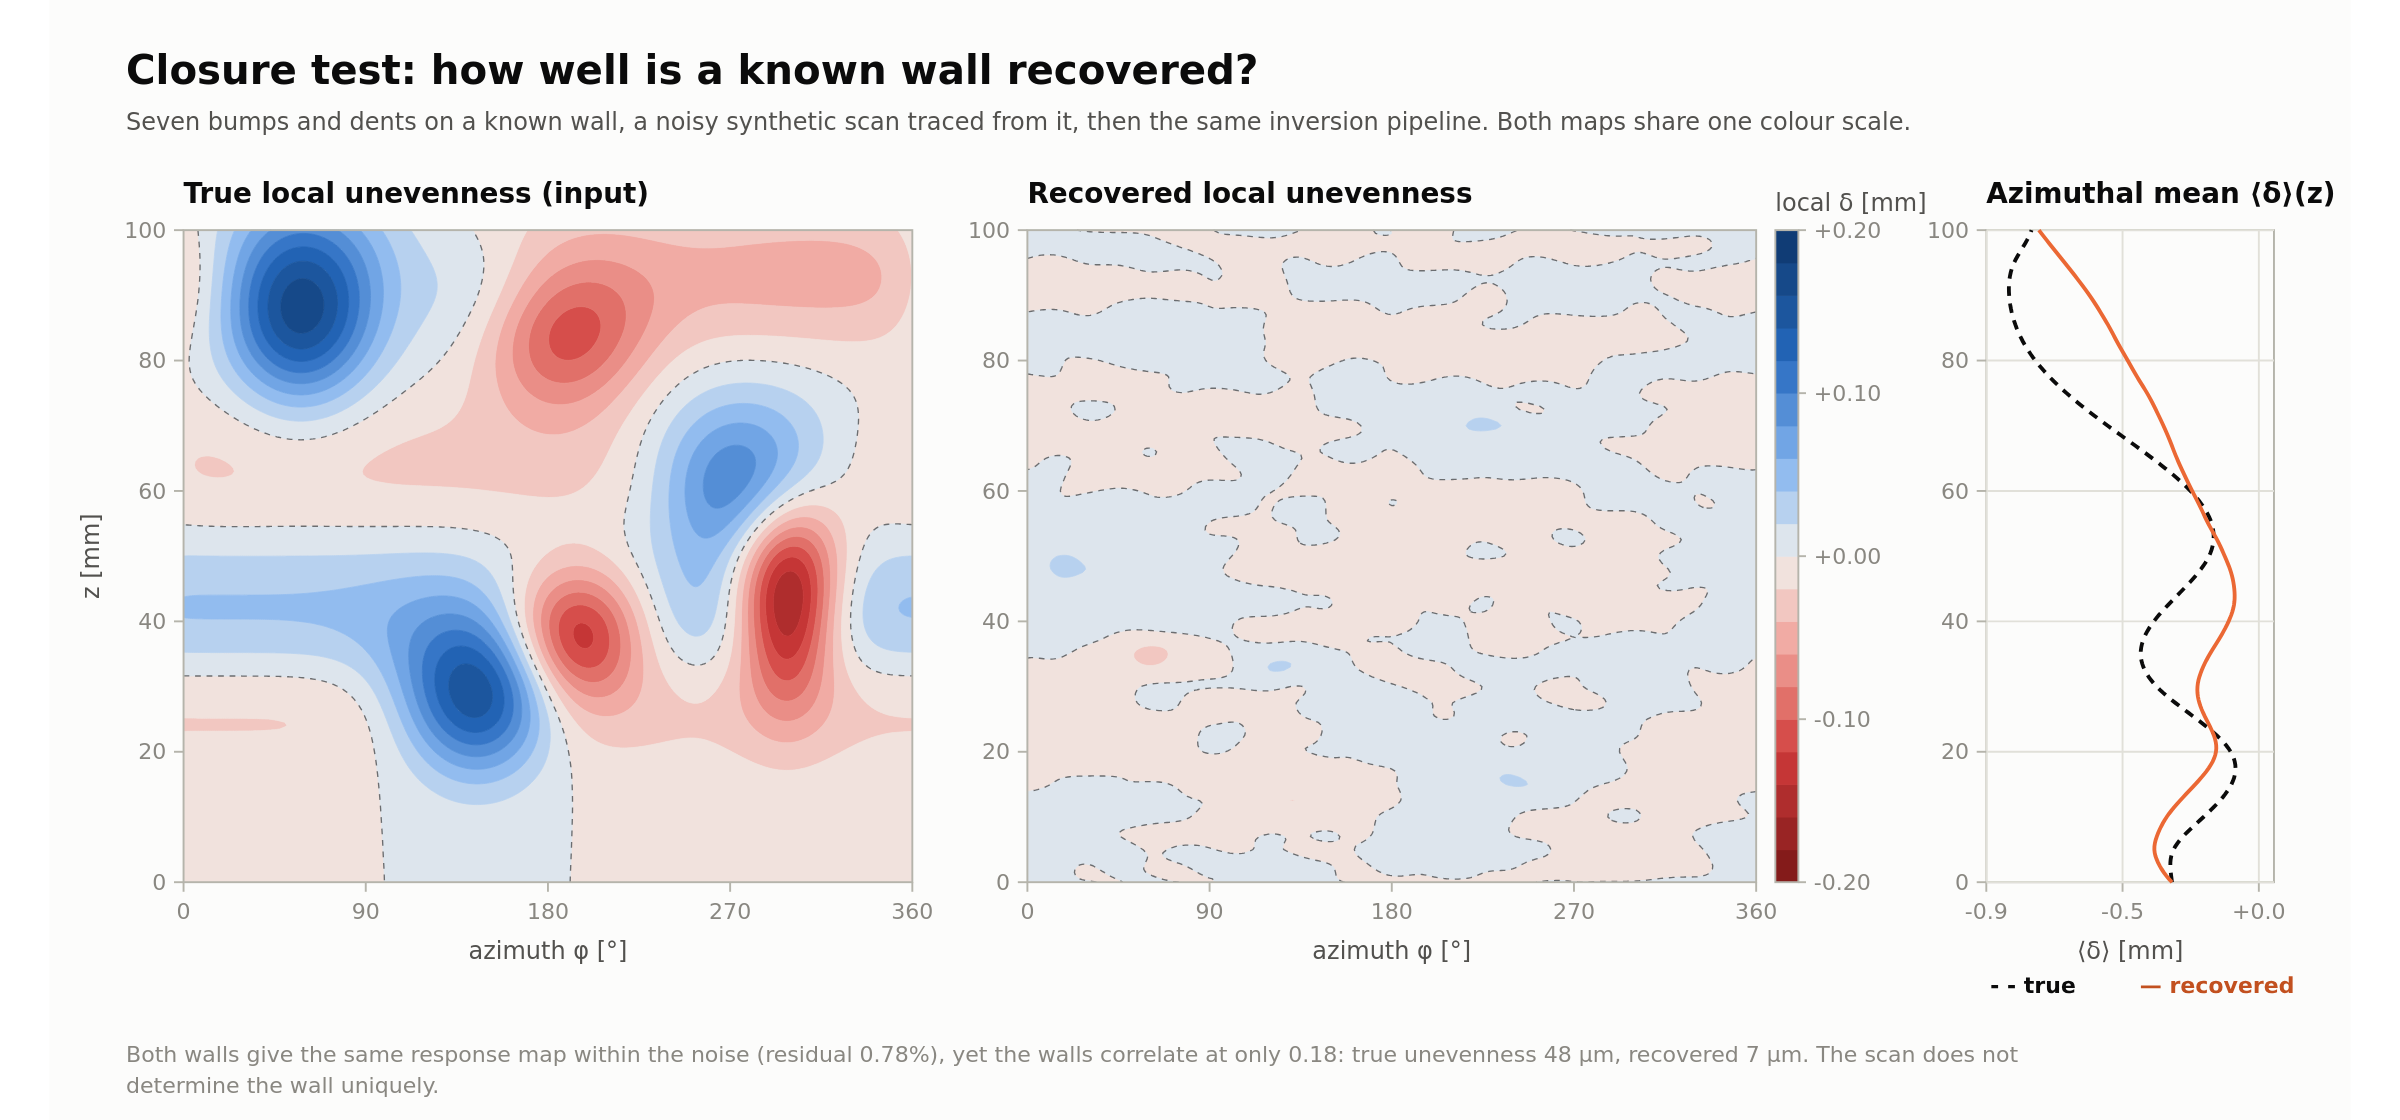
\includegraphics[width=\textwidth]{fig/en/closure.png}
\caption{Closure test. Left: the true local unevenness put in. Middle: the unevenness recovered from
the synthetic scan, on the same colour scale. Right: azimuthal mean profiles. Both walls give the same
response map within the noise.}\label{fig:closure}
\end{figure}

The outcome (Figure~\ref{fig:closure}) has two parts and both matter. The synthetic map is reproduced
to the noise: residual \ClMapRms\,\%, $\chi^2/N=\ClChiTwo$. The chain can therefore reach the noise
level when the truth lies inside the model. The wall is a different matter: true and recovered
local unevenness are only weakly correlated, at \ClCorrAll{} (1 would be a perfect recovery), the recovered
amplitude is \ClRmsRec\um{} against \ClRmsTrue\um{} true, their difference is \ClRmsErr\um, and the
azimuthal mean profile is off by \ClProfErr\um{} RMS with a mean offset of \ClProfBias\um. All these
are root mean squares: a bias counts.

\subsection{Resolution study}
\label{sec:resolution}

\begin{lstlisting}
python study_resolution.py cl1b ../out/synth_cl1.npz ../out/fitB_cl1b.npz
\end{lstlisting}
The Jacobian, linearised around the axisymmetric base wall, is decomposed by singular values after
the direction of the map itself has been projected out (the overall amplitude is a free parameter of
every fit). The decomposition orders the wall patterns by how strongly they change the scan. The scan
fixes the amplitude of pattern $k$ to $\pm\sigma_T/s_k$ (one standard deviation), with $s_k$ its
singular value and $\sigma_T$ the noise of one scan point in transmission units.
Table~\ref{tab:res} gives, for the $k$ best-determined patterns, that uncertainty for pattern $k$
expressed as the RMS height of the pattern on the wall surface, the share of the true test wall's
deformation power that lies in them, the correlation between the true and the recovered wall inside
them, and the ratio of the recovered to the true amplitude there.

\begin{table}[H]
\centering
\caption{What the scan determines (closure test). For the $k$ best-determined patterns: one-sigma
uncertainty of the amplitude of pattern $k$ as surface RMS, share of the true wall's deformation
power, correlation of recovered and true wall, ratio of recovered to true amplitude. The singular
values fall smoothly, by three orders of magnitude over the 1032 patterns.}\label{tab:res}
\begin{tabular}{@{}rrrrr@{}}
\toprule
Best $k$ & Uncertainty [\textmu m] & Share [\%] & Correlation & Amplitude ratio \\
\midrule
\ResolutionRows
\bottomrule
\end{tabular}
\end{table}

The singular values fall smoothly: there is no sharp boundary between patterns the scan sees and
patterns it does not, and no single number of visible patterns. With explicit cut-offs: inside the
best 30 patterns the recovered and the true wall correlate at \ResCThirty, and these patterns hold
\ResFThirty\,\% of the test wall's deformation power; inside the best 100 the correlation is
\ResCHundred{} (\ResFHundred\,\%), inside the best 150 it is \ResCOneFifty{} (\ResFOneFifty\,\%).
Correlation alone hides amplitude errors: inside the best 100 patterns the recovered amplitude is
\ResAHundred{} times the true one. The best-determined patterns are fixed to well below a
micrometre of surface RMS (\ResSThirty\um{} for pattern 30, \ResSHundred\um{} for pattern 100), but
they hold little of the deformation of a wall with broad, gentle bumps. The supported statement is
therefore: the wall is recovered well only inside roughly the 100 best-determined combinations, which
hold about \ResFHundred\,\% of the true deformation.

Four caveats. The Jacobian used here is the one of the kernels, which is poor for broad smooth shapes
and for the mean profile (Section~\ref{sec:jactest}); the figures of Table~\ref{tab:res} are therefore
indicative, not precise. The analysis is linear, around the axisymmetric base wall, not around the
fitted wall. The patterns are orthonormal in the metric of the spline-coefficient vector, not in a metric of
the surface. And where a pattern drops out of sight depends on its amplitude, so any cut-off $k$ is a
choice.

\subsection{Two fits of the measured scan}
\label{sec:prev}

\begin{lstlisting}
python compare_walls.py ../out/final_data.npz ../results/earlier/wall_coeffs_cb81f08.json
\end{lstlisting}
The closure test shows the non-uniqueness on a synthetic scan. This check shows it on the measured
one. \path{results/earlier/wall_coeffs_cb81f08.json} holds the wall that was published with an
earlier version of the toolkit (commit \code{cb81f08}), before the march and the ray sequence of the
tracer were corrected. The script traces that wall with the present tracer, aperture and light spot
(20\,000 rays per point by default; third argument), fits its amplitude as \code{final.py} does, and
compares it with the wall of the present result. It writes \path{../out/compare_prev.json}, which
\code{collect\_numbers.py} copies into the block \code{prev} of \code{numbers.json}; \code{run\_all.sh}
runs it right after the pipeline. Both walls must be on the same spline grid.

\begin{tabularx}{\textwidth}{@{}L{3.6cm}L{3.2cm}Y@{}}
\toprule
Field & Value & Meaning \\
\midrule
\code{rms\_earlier}, \code{rms\_now} & \PrevRmsEarlier\,\%, \PrevRmsNow\,\% & data minus simulation in the inner aperture, earlier and present wall \\
\code{map\_diff} & \PrevMapDiff\,\% & RMS difference of the two simulated maps \\
\code{corr\_local} & \PrevCorr & correlation of the local unevenness (azimuthal mean removed), whole wall \\
\code{bands} & \PrevCorrEntrance; \PrevCorrRest & the same in five 20\,mm bands of $z$, from the entrance to the exit \\
\code{loc\_rms\_earlier}, \code{loc\_rms\_now}, \code{loc\_diff} & \PrevLocRms, \LocRmsOne, \PrevLocDiff\um & RMS local unevenness of the two walls and of their difference \\
\code{prof\_diff}, \code{prof\_diff\_max} & \PrevProfDiff, \PrevProfDiffMax\um & RMS and largest difference of the azimuthal mean profiles \\
\bottomrule
\end{tabularx}

How to read it. The two walls fit the measured scan equally well, and their simulated maps differ by
much less than either differs from the data. If the scan determined the wall, the two would agree.
They agree only in the first 20\,mm behind the entrance (correlation \PrevCorrEntrance); further in,
the local unevenness is uncorrelated or even opposite, the difference of the two (\PrevLocDiff\um{}
RMS) is larger than either unevenness, and the mean profiles differ by up to \PrevProfDiffMax\um.
A correlation near 1 here would be a necessary sign of a determined wall, not a sufficient one; the
low value found is direct evidence, on the measured data, that the wall is not determined. The two
fits are not independent samples of all walls that fit (same method, same regularisation, same start
recipe), so the spread between them is a lower bound on the freedom the scan leaves.

\subsection{Further studies}

\begin{tabularx}{\textwidth}{@{}L{4.7cm}Y@{}}
\toprule
Script & Purpose \\
\midrule
\code{study\_deformations.py} & response maps for a set of simple test deformations (barrel, hourglass,
single bumps, entrance flare, exit pinch) \\
\code{study\_reflectivity.py} & radial profile of the ideal cone for mirror reflectivities below 1,
against the data \\
\code{study\_launch\_cone.py} & checks that the launch-angle cut \code{smax} loses no detected light \\
\code{look\_data.py} & quick plots of the raw scan \\
\bottomrule
\end{tabularx}

% ====================================================================== 7
\section{Outputs and file formats}

\subsection{Input scan}

\path{data/scan_summary.csv} has one line per scan point with the columns \code{idx\_x},
\code{idx\_y}, \code{direction}, \code{cmd\_x\_mm}, \code{cmd\_y\_mm}, \code{pos\_x\_mm},
\code{pos\_y\_mm}, \code{timestamp}, \code{n\_events}, \code{n\_saved}, \code{probe\_V},
\code{passed}, \code{acq\_time\_s}. The grid indices \code{idx\_x}, \code{idx\_y} place each point;
the code uses the positions \code{pos\_x\_mm}, \code{pos\_y\_mm}, the signal \code{probe\_V}
(volts) and the flag \code{passed}. The grid must be regular and complete.

\subsection{Intermediate files in \texttt{out/}}

\begin{tabularx}{\textwidth}{@{}L{3.5cm}Y@{}}
\toprule
File & Arrays \\
\midrule
\code{edge.npz} & \code{cx}, \code{cy} centre (stage coordinates); \code{ped}, \code{ped\_rms}
pedestal; \code{fourier[9,2]} cosine and sine coefficients ($m=0\ldots8$) of $r_\mathrm{ap}(\varphi)$;
\code{phi}, \code{r\_edge}, \code{sigma}, \code{level} per-sector edge fits; \code{spot\_radius},
\code{dr\_disc} from \code{edge\_spot.py} \\
\code{A\_<tag>.npz} & \code{p} profile coefficients (and the reflectivity if fitted); \code{NZ};
\code{rho}, \code{dat}, \code{err}, \code{T}, \code{A} the fitted radial profile; \code{zz},
\code{d0} the profile $\delta_0(z)$ \\
\code{start\_<tag>.npz} & \code{c[24, NZ+3]}, \code{NZ}, \code{NPHI}, \code{refl} \\
\code{kmodes\_<tag>.npz} & \code{A[nk, 13, 3, nrho]} harmonic amplitudes; \code{QS[13,3]} the
harmonics $q$ of each mode ($-1$ = unused); \code{rho}; \code{p} base profile; \code{T0} base map;
\code{NPHI}, \code{NZ}, \code{refl} \\
\code{fitB\_<tag>.npz} & \code{c[24, 43]} fitted coefficients; \code{base}; \code{A} amplitude;
\code{hist} ($\chi^2/N$, residual, amplitude per iteration); \code{T}, \code{xs}, \code{ys},
\code{dat} model, positions and data of the fitted points; \code{lam}, \code{NPHI}, \code{NZ},
\code{refl} \\
\code{final\_<tag>.npz} & \code{x}, \code{y} scan axes; \code{S[nx,ny]} pedestal-subtracted data;
\code{M} model; \code{T} transmission; \code{Mideal} ideal cone; \code{A}; \code{R} distance from the
centre; \code{cx}, \code{cy}; \code{phi[361]}, \code{z[201]}, \code{DEL[361,201]} the wall on a grid;
\code{c}; \code{refl}; \code{mc} model noise \\
\code{synth\_<tag>.npz} & \code{S} synthetic scan; \code{c\_true[48,23]}; \code{bumps}; \code{A};
\code{fourier[25,2]} aperture of the synthetic wall; \code{seed}; \code{base\_sha1} fingerprint of the
profile it is built from \\
{\small\code{pipeline\_<tag>.log}} & full output of every step of \code{pipeline.sh} \\
\code{ideal\_cone.json}, \code{gpu\_check.json}, \code{recip.json} & results of
\code{test\_ideal\_cone.py}, \code{test\_gpu\_vs\_cpu.py}, \code{test\_reciprocity.py}; the last two
with the fingerprint \code{wall\_sha1} of the wall \\
\code{g4\_compare.json}, \code{g4\_ideal.json} & Geant4 against the tracer for the fitted wall and
the ideal cone (\code{ratio}, \code{ratio\_err}, \code{pull\_rms}, \code{corr}, \code{spot},
\code{refl}, \code{wall\_sha1}) \\
\code{resolution.json} & resolution study: \code{k}, \code{corr}, \code{amp\_ratio},
\code{frac\_true}, \code{amin\_um}, \code{amin\_surf\_um}, \code{corr\_all}, \code{base\_sha1} \\
\code{A\_refl.npz} & Stage A with the mirror reflectivity free, started from \code{A\_data.npz}
(\code{run\_all.sh --with-checks}) \\
\code{jacobian.json}, \code{test\_jacobian.log} & \code{test\_jacobian.py}: kernels against exact
changes of the map (Section~\ref{sec:jactest}); the JSON file carries \code{wall\_sha1}. The logs of
the two runs quoted in this manual are tracked in \path{results/checks/} \\
\code{compare\_prev.json} & \code{compare\_walls.py}: this wall against the wall of an earlier fit
(Section~\ref{sec:prev}), with \code{wall\_sha1} and \code{earlier\_sha1} \\
\bottomrule
\end{tabularx}

\subsection{Results}

\code{wall\_delta.csv}: three comment lines, then the columns \code{phi\_deg} (0--359, step 1),
\code{z\_mm} (0--100, step 0.5), \code{r\_cad\_mm}, \code{delta\_mm}, \code{delta\_azimuthal\_mean\_mm},
\code{delta\_local\_mm}.

\code{wall\_coeffs.json}: \code{NPHI}, \code{NZ} and the coefficient matrix \code{c[NPHI][NZ+3]} in
mm. It can be fed back to the tracer:
\begin{lstlisting}
import json, numpy as np, lgtrace as lg
c = np.array(json.load(open('../results/wall_coeffs.json'))['c'])
T = lg.transmission([0.0, 2.0], [0.0, -1.0], coeffs=c, nray=20000, smax=0.55, sig=-0.34)
\end{lstlisting}
\code{sig} $<0$ is a disc of radius $-$\code{sig}; \code{sig} $>0$ a Gaussian sigma; positions are
relative to the aperture centre.

\path{results/earlier/wall_coeffs_cb81f08.json}: the wall published with an earlier version of the
toolkit, in the format of \code{wall\_coeffs.json}; the reference of \code{compare\_walls.py}.

\code{numbers.json}: the fingerprint of the wall (\code{wall\_sha1}), the fit quality (\code{rms},
\code{bias}, \code{rms\_id}, \code{chi2}, \code{corr}, \code{rms\_ring}, \code{bias\_ring},
\code{ring\_worst}, \code{excess}, in percent of the plateau; \code{ring\_worst} is the most negative
azimuthal mean of data minus simulation in the 0.1\,mm annuli between 8.0 and 8.5\,mm), the noise (\code{noise} of one scan point, \code{mc\_noise}
of the model map, in percent), the wall statistics (\code{loc\_rms}, \code{loc\_min}, \code{loc\_max}
in \textmu m; \code{mean\_min}, \code{mean\_max} in mm), the aperture (\code{r\_ap}, \code{spot\_r}),
and one block per check that has been run: \code{ideal}, \code{g4\_ideal}, \code{g4}, \code{gpu},
\code{recip}, \code{jacobian} (\code{corr\_min}, \code{corr\_max}, \code{slope\_min}, \code{slope\_max}
for the non-axisymmetric perturbations; \code{m0\_step\_corr\_min/max}, \code{m0\_smooth\_corr\_min/max},
\code{m0\_smooth\_mean\_min/max} for the axisymmetric ones), \code{refl\_fit}, \code{prev},
\code{closure}, \code{resolution}. Every ``rms'' is a root mean
square, with the bias given separately where it matters. A block carries \code{current}: true if the
check was run on the wall of this result, false if its file is left over from an earlier
reconstruction.

Geant4 mesh (\code{mesh.txt}): first line ``\code{NPHI NZ}''; then \code{NZ} lines, each with $z$ and
the \code{NPHI} wall radii at $\varphi_i=2\pi i/\code{NPHI}$, in mm.

% ====================================================================== 8
\section{Adapting the toolkit to another light guide or scan}
\label{sec:adapt}

\textbf{Geometry.} The cone is defined by three constants, which appear in four places and must agree:
\begin{itemize}
\item \path{src/lgtrace.py}: \code{R1, R2, L} (and \code{SLOPE} derived from them);
\item \path{src/lgcl.py}: the macros \code{R1}, \code{LEN}, \code{SLOPE} in the OpenCL source
(\code{SLOPE} is written out as a number);
\item \path{web/lgtrace.js}: \code{R1, R2, L} for the browser demonstration;
\item \path{g4/lgsim.cc}: \code{R1, R2, LEN}, and the sizes of the world box and of the two photon
dumps if the guide is much larger.
\end{itemize}
\code{export\_wall.py} and \code{make\_ray\_svg.py} also write out $r_\mathrm{CAD}=8.75-0.0475\,z$.
A shape that is not a straight cone needs a different reference surface in the functions \code{\_f}
and \code{\_fg} and in the bounding-cone bracket; the B-spline part carries over unchanged.

\textbf{Scan.} Any regular rectangular grid works. Either provide a CSV with the same columns and
point \code{LG\_SCAN} to it, or edit \code{load()} in \path{src/load_scan.py}; it must return the axes
\code{x}, \code{y} and the signal \code{V[ix, iy]}. In \path{src/edge.py} set the first guess of the
centre and the radial windows used for the pedestal ($r>10$) and for the edge fit ($7.6<r<9.6$).

\textbf{Fit radius.} \code{LG\_RCUT} (8.0\,mm) must stay inside the aperture by more than the spot
radius, so that the spot is never clipped at a fitted point. The polar grid in
\code{kernel\_modes.py} (57 radii of 0.15\,mm) must cover it.

\textbf{Launch cone.} \code{smax} must exceed the largest $\sin\theta$ of any detected ray, roughly
$R_2/R_1$ plus a margin. Check with \code{study\_launch\_cone.py}. Too small a value silently loses
light; too large a value only costs time.

\textbf{Resolution of the wall.} $N_\varphi$ is an argument of \code{kernel\_modes.py} and
\code{refine.py} writes 24 azimuthal knots for a Stage-A input; $N_z$ is the second argument of
\code{refine.py}. Finer grids resolve thinner arcs but add poorly constrained parameters; cost grows
with $N_z\times(N_\varphi/2+1)$ kernel runs.

\textbf{Regularisation.} $\lambda$ is the third argument of \code{stageB.py}. With the damped
iterations the result depends weakly on it: the fit stays close to the start wall anyway. To see the
effect of the prior, change the start wall rather than $\lambda$.

\textbf{Noise and statistics.} The point noise of the scan (\code{SIGD} in \code{stageB.py}, also
used in \code{final.py} and \code{collect\_numbers.py}) is $2.0\times10^{-4}$\,V for the shipped data;
estimate it for new data from the high-pass residual of the plateau. Rays per point: 12\,000 for the
kernels, 20\,000 per iteration, 40\,000 for the final map. Halving them roughly halves the run time
and raises the model noise by 30--40\,\%.

% ====================================================================== 9
\section{Limits and interpretation}
\label{sec:limits}

\textbf{The solution is not unique.} Different walls give the same response map within the noise.
Two fits of the measured scan reproduce it equally well (\PrevRmsEarlier\,\% and \PrevRmsNow\,\%) with
walls that agree only close to the entrance: correlation \PrevCorr{} overall, \PrevCorrEntrance{} in
the first 20\,mm (Section~\ref{sec:prev}). In the closure test the true wall is recovered well only
inside roughly the 100 shape combinations the scan determines best (correlation \ResCHundred), which
hold \ResFHundred\,\% of the true deformation (Table~\ref{tab:res}); a wall with broad, gentle bumps
0.15--0.3\,mm high (\ClRmsTrue\um{} RMS) and the recovered wall with \ClRmsRec\um{} RMS fit the same
synthetic scan equally well. The wall shown is one regularised solution: the fit penalises unevenness and its
damped iterations stay near the axisymmetric start wall, so it tends towards a smooth wall. It is not
shown to be the least uneven wall that fits, since the stopping rule proves no minimum and $Q$ is not
the surface RMS. The local unevenness of \LocRms\um{} RMS shows that little unevenness is enough to
explain the scan. It is neither an estimate of what the real wall has nor a bound on it from below:
part of the structure could come from reflectivity or detector non-uniformity instead of geometry.

\textbf{The azimuthal mean profile is poorly fixed.} It is strongly degenerate with the overall signal
scale, with the exit radius and with the mirror reflectivity, and different fits return different
profiles. The present profile and that of the earlier wall are \PrevProfDiff\um{} RMS apart, up to
\PrevProfDiffMax\um, while both fit equally well; in the closure test the recovered profile is off by
\ClProfErr\um{} RMS; with the reflectivity free the axisymmetric fit moves to $R=\ReflFit$ and another
profile. The linear kernels are poor for changes of the mean profile (Section~\ref{sec:jactest}), so
the fit finds such steps inefficiently. Common to all fits are only the entrance radius (\RAp\,mm, measured directly from the scan
edge) and a bore that is narrower than CAD along the whole length. The local unevenness is
\LocRmsOne\um{} RMS here and \PrevLocRms\um{} in the earlier wall; a still earlier fit from another
starting point gave 44\um. All reproduce the scan to about 1\,\%.

\textbf{Everything is attributed to geometry.} By assumption the mirror reflectivity is 1, the PMT
response is uniform in position and angle, and the source is an ideal Lambertian disc. Real
reflectivity variations, the seam of the reflective film, dust, or photocathode non-uniformity would
all be read as wall unevenness.

\textbf{Unexplained structure.} The fit to the shipped scan ends at $\chi^2/N=\ChiTwo$, not 1: a few
tenths of a percent of correlated structure on a 1\,mm scale is not explained by this fit. The
closure test shows that the chain can reach the noise when the truth lies inside the model. It does
not show that the fit of the shipped scan is the best one the model allows: two earlier fits of the
same scan, with earlier versions of the code, ended at $\chi^2/N=1.48$ and 1.31, so the value depends
on the start, the settings and the code version. The
remainder may be structure outside the model (smooth wall, perfect mirror, uniform detector), an
unfinished optimisation, or both. $\chi^2/N$ is not a calibrated goodness of fit, because the
effective number of fitted parameters is unknown.

\textbf{The entrance rim.} Between $r=8.0$\,mm and the aperture edge (\RAp\,mm) the measurement lies
below the model. Over the ring from 8.0 to 8.5\,mm the residual is about \RmsRing\,\% RMS per point
with a mean of \BiasRing\,\% of the plateau, and the azimuthal mean reaches \RingWorst\,\% in the worst
0.1\,mm annulus. The measured signal drops earlier
than the model inside the aperture but has no tail outside, as if a band about 0.1\,mm wide at the rim
were lossy (a chamfer, or film that stops short of the edge). This is below the resolution of the
model and the ring is excluded from the fit.

\textbf{Resolution.} The deviation field has 2.5\,mm cells along the axis and $15^\circ$ in azimuth
(2.2\,mm of arc at the entrance, 1.0\,mm at the exit). Finer structure is smoothed.

\textbf{Orientation of the azimuth.} $\varphi$ follows the scan axes. Whether the figure is a mirror
image of the hardware depends on the stage orientation.

\textbf{What would pin down the real wall.} Independent information, each piece constraining a
further set of shape combinations:
\begin{itemize}
\item scans with a collimated beam at several incidence angles (each angle selects different ray
families, where the diffuse source averages over all of them);
\item angle-resolved or position-resolved readout at the exit instead of one integrating PMT;
\item a scan from the exit side;
\item direct profilometry of the wall, or a coordinate measurement of the bore at a few heights, to
fix the azimuthal mean.
\end{itemize}
The resolution study (\code{study\_resolution.py}) can be repeated for a simulated additional
measurement to see how many more patterns it would make visible before taking the data.

% ====================================================================== 10
\section{Troubleshooting}

\trouble{\code{IndexError} or ``no devices'' when the GPU tracer starts}{\code{pyopencl} found no GPU device. Check \code{clinfo -l}; make sure the user is in the
\code{render} and \code{video} groups; on AMD check that the ROCm OpenCL ICD is installed. To run
without a GPU set \code{LG\_GPU=0}.}
\trouble{The desktop stutters or the GPU driver resets during a run}{The tracer submits slices of about 0.6\,s (\code{slice\_s} in \code{lgcl.transmission}). Lower it if
the GPU is shared with interactive work. Run only one GPU job at a time.}
\trouble{Results change after editing \code{lgtrace.py}, or \code{numba} complains about a cached function}{Delete \path{src/__pycache__}. The compiled functions are cached there and rebuilt on the next run
(a few seconds).}
\trouble{A driver stops with ``step failed'' or a FAIL line}{The shell drivers stop at the first failing step or self-test. \code{pipeline.sh} prints the end
of \path{out/pipeline_<tag>.log}; the full output of the step is in that file.}
\trouble{A job dies with exit code 137, or ``Killed''}{It exceeded the memory limit of the wrapper. The pipeline needs less than 1\,GB; a Geant4 job with
the 720\,000-facet mesh about 0.7\,GB. Raise the limit with \code{LG\_MEM=12G} only if the job is
known to need it.}
\trouble{``no improving step; stop'' in the first iteration}{See Section~\ref{sec:pipeline}: raise \code{LG\_MU}, or recompute the kernels around the current wall.
At the end of a run the message is the normal stopping rule.}
\trouble{\code{stageB.py} stops, then the final $\chi^2$ is higher}{\code{final.py} uses a different seed and more rays; differences of a few hundredths in $\chi^2/N$
are Monte Carlo noise. Larger differences mean the fit followed the noise of its own ray set; raise
\code{LG\_NRAY}.}
\trouble{The manual figures come out empty, or Firefox refuses to start}{Another Firefox is using the same profile. \code{make\_manual\_figs.sh} keeps a private profile in
\path{docs/manual/.ffprofile}; delete that directory and run again.}
\trouble{Geant4: ``Overlapping daughter with mother volume''}{The world box in \code{lgsim.cc} must contain the cavity and both photon dumps; enlarge it when the
guide is longer than 100\,mm.}
\trouble{Geant4: ``Particle e- without a Process Manager''}{This appears when \code{G4OpticalPhysics} is registered alone. Keep the minimal physics list of
\code{lgsim.cc}: the optical photon only, with transportation and the optical boundary process
(\code{G4OpBoundaryProcess}).}
\trouble{Geant4 is very slow}{Tracking in the tessellated solid costs about 10\,ms per photon whatever the mesh size between
180\,000 and 720\,000 facets. Use few points with a few thousand photons, in parallel processes.}

% ====================================================================== 11
\section{Resource policy: \texttt{tools/run\_limited.sh}}
\label{sec:resources}

The development machine is shared, so every long or parallel job is started through a wrapper that
keeps it from exhausting the memory and makes it yield the CPU to other work.
\begin{lstlisting}
tools/run_limited.sh <command> [arguments...]
tools/run_limited.sh --cores        # print the number of cores a job would get now
\end{lstlisting}
\begin{itemize}
\item One invocation is one transient \code{systemd} user scope with \code{MemoryMax} (default
6\,GB) and no swap: a job that exceeds the limit is killed.
\item The number of cores is chosen when the job starts: all cores, minus those busy with other work,
minus four spare, clamped to the range 2--24. It sets the CPU quota of the scope and the thread
counts of \code{numba}, OpenMP and BLAS.
\item The job runs at \code{nice 19} with idle I/O priority and a CPU weight of 10, so other work
gets the CPU first.
\item \code{LG\_GPU=1} is exported, so tracing runs on the GPU unless \code{LG\_GPU=0} is given.
\end{itemize}
Overrides: \code{LG\_MEM=12G}, \code{LG\_CPUS=8}, \code{LG\_GPU=0} in front of the command. On a
machine without \code{systemd} user sessions run the commands directly and set \code{LG\_GPU=1} and
\code{NUMBA\_NUM\_THREADS} by hand.

What the wrapper does not do. The limits apply to one invocation: jobs started side by side each get
their own scope and their own limits, so parallel work that needs a total cap must be started from
inside \emph{one} invocation. \code{g4/run\_final.sh} does that for its Geant4 processes. And a
cgroup memory limit does not cap GPU allocations: the GPU is outside the cgroup accounting. The
tracer therefore limits itself, with host buffers of a few megabytes and sub-second slices. Run one
GPU job at a time.

% ====================================================================== 12
\section{Author, contact, license and citation}

LGWallRecon was written by Hengne Li (李衡讷), South China Normal University.

Contact: \code{Hengne.Li@cern.ch}, \code{Hengne.Li@m.scnu.edu.cn}.

Repositories:
\begin{itemize}
\item GitHub: \GithubURL
\item GitLab (SCNU group): \GitlabURL
\end{itemize}

License: LGWallRecon is released under the MIT License, Copyright (c) 2026 Hengne Li (李衡讷).
You may use, copy, modify and redistribute it, including the measured scan and the CAD file in
\path{data/}, provided the copyright and permission notice is kept. It comes without warranty.
The full text is in the file \path{LICENSE} at the top of the repository.

To cite the toolkit:
\begin{quote}
Hengne Li, \emph{LGWallRecon: light-guide inner-wall reconstruction from an entrance-face scan},
software, 2026.\\
\GithubURL
\end{quote}

When quoting results obtained with it, state the assumptions of the model (perfect specular wall,
uniform detector, Lambertian source) and that the reconstructed wall is one regularised solution
of a non-unique inverse problem.

\end{document}
